\documentclass[twoside]{book}

% Packages required by doxygen
\usepackage{calc}
\usepackage{doxygen}
\usepackage{graphicx}
\usepackage[utf8]{inputenc}
\usepackage{makeidx}
\usepackage{multicol}
\usepackage{multirow}
\usepackage{textcomp}
\usepackage[table]{xcolor}

% Font selection
\usepackage[T1]{fontenc}
\usepackage{mathptmx}
\usepackage[scaled=.90]{helvet}
\usepackage{courier}
\usepackage{amssymb}
\usepackage{sectsty}
\renewcommand{\familydefault}{\sfdefault}
\allsectionsfont{%
  \fontseries{bc}\selectfont%
  \color{darkgray}%
}
\renewcommand{\DoxyLabelFont}{%
  \fontseries{bc}\selectfont%
  \color{darkgray}%
}

% Page & text layout
\usepackage{geometry}
\geometry{%
  a4paper,%
  top=2.5cm,%
  bottom=2.5cm,%
  left=2.5cm,%
  right=2.5cm%
}
\tolerance=750
\hfuzz=15pt
\hbadness=750
\setlength{\emergencystretch}{15pt}
\setlength{\parindent}{0cm}
\setlength{\parskip}{0.2cm}
\makeatletter
\renewcommand{\paragraph}{%
  \@startsection{paragraph}{4}{0ex}{-1.0ex}{1.0ex}{%
    \normalfont\normalsize\bfseries\SS@parafont%
  }%
}
\renewcommand{\subparagraph}{%
  \@startsection{subparagraph}{5}{0ex}{-1.0ex}{1.0ex}{%
    \normalfont\normalsize\bfseries\SS@subparafont%
  }%
}
\makeatother

% Headers & footers
\usepackage{fancyhdr}
\pagestyle{fancyplain}
\fancyhead[LE]{\fancyplain{}{\bfseries\thepage}}
\fancyhead[CE]{\fancyplain{}{}}
\fancyhead[RE]{\fancyplain{}{\bfseries\leftmark}}
\fancyhead[LO]{\fancyplain{}{\bfseries\rightmark}}
\fancyhead[CO]{\fancyplain{}{}}
\fancyhead[RO]{\fancyplain{}{\bfseries\thepage}}
\fancyfoot[LE]{\fancyplain{}{}}
\fancyfoot[CE]{\fancyplain{}{}}
\fancyfoot[RE]{\fancyplain{}{\bfseries\scriptsize Generated on Wed Mar 26 2014 22\-:31\-:27 for Axiom Enterprises -\/ Route Logistics by Doxygen }}
\fancyfoot[LO]{\fancyplain{}{\bfseries\scriptsize Generated on Wed Mar 26 2014 22\-:31\-:27 for Axiom Enterprises -\/ Route Logistics by Doxygen }}
\fancyfoot[CO]{\fancyplain{}{}}
\fancyfoot[RO]{\fancyplain{}{}}
\renewcommand{\footrulewidth}{0.4pt}
\renewcommand{\chaptermark}[1]{%
  \markboth{#1}{}%
}
\renewcommand{\sectionmark}[1]{%
  \markright{\thesection\ #1}%
}

% Indices & bibliography
\usepackage{natbib}
\usepackage[titles]{tocloft}
\setcounter{tocdepth}{3}
\setcounter{secnumdepth}{5}
\makeindex

% Hyperlinks (required, but should be loaded last)
\usepackage{ifpdf}
\ifpdf
  \usepackage[pdftex,pagebackref=true]{hyperref}
\else
  \usepackage[ps2pdf,pagebackref=true]{hyperref}
\fi
\hypersetup{%
  colorlinks=true,%
  linkcolor=blue,%
  citecolor=blue,%
  unicode%
}

% Custom commands
\newcommand{\clearemptydoublepage}{%
  \newpage{\pagestyle{empty}\cleardoublepage}%
}


%===== C O N T E N T S =====

\begin{document}

% Titlepage & ToC
\hypersetup{pageanchor=false}
\pagenumbering{roman}
\begin{titlepage}
\vspace*{7cm}
\begin{center}%
{\Large Axiom Enterprises -\/ Route Logistics \\[1ex]\large 0.\-2 }\\
\vspace*{1cm}
{\large Generated by Doxygen 1.8.6}\\
\vspace*{0.5cm}
{\small Wed Mar 26 2014 22:31:27}\\
\end{center}
\end{titlepage}
\clearemptydoublepage
\tableofcontents
\clearemptydoublepage
\pagenumbering{arabic}
\hypersetup{pageanchor=true}

%--- Begin generated contents ---
\chapter{Namespace Index}
\section{Namespace List}
Here is a list of all namespaces with brief descriptions\-:\begin{DoxyCompactList}
\item\contentsline{section}{\hyperlink{namespacebasic__window}{basic\-\_\-window} }{\pageref{namespacebasic__window}}{}
\item\contentsline{section}{\hyperlink{namespacehello}{hello} }{\pageref{namespacehello}}{}
\item\contentsline{section}{\hyperlink{namespacepython__client__test}{python\-\_\-client\-\_\-test} }{\pageref{namespacepython__client__test}}{}
\item\contentsline{section}{\hyperlink{namespacepython__server__test}{python\-\_\-server\-\_\-test} }{\pageref{namespacepython__server__test}}{}
\end{DoxyCompactList}

\chapter{Hierarchical Index}
\section{Class Hierarchy}
This inheritance list is sorted roughly, but not completely, alphabetically\-:\begin{DoxyCompactList}
\item \contentsline{section}{account}{\pageref{structaccount}}{}
\item \contentsline{section}{Connection$<$ Type $>$}{\pageref{classConnection_3_01Type_01_4}}{}
\item \contentsline{section}{Linked\-List$<$ Type $>$}{\pageref{classLinkedList}}{}
\item \contentsline{section}{Linked\-List$<$ Location $>$}{\pageref{classLinkedList}}{}
\item \contentsline{section}{Linked\-List$<$ Py\-Func $>$}{\pageref{classLinkedList}}{}
\item \contentsline{section}{location}{\pageref{structlocation}}{}
\item \contentsline{section}{Location}{\pageref{classLocation}}{}
\begin{DoxyCompactList}
\item \contentsline{section}{Node$<$ Location $>$}{\pageref{classNode}}{}
\end{DoxyCompactList}
\item \contentsline{section}{Matrix}{\pageref{classMatrix}}{}
\item \contentsline{section}{Py\-Func$<$ Type $>$}{\pageref{classPyFunc}}{}
\begin{DoxyCompactList}
\item \contentsline{section}{Node$<$ Py\-Func $>$}{\pageref{classNode}}{}
\item \contentsline{section}{Return\-List$<$ Type $>$}{\pageref{classReturnList}}{}
\end{DoxyCompactList}
\item \contentsline{section}{Py\-I}{\pageref{classPyI}}{}
\item \contentsline{section}{Salesman}{\pageref{classSalesman}}{}
\item Type\begin{DoxyCompactList}
\item \contentsline{section}{Node$<$ Type $>$}{\pageref{classNode}}{}
\end{DoxyCompactList}
\end{DoxyCompactList}

\chapter{Class Index}
\section{Class List}
Here are the classes, structs, unions and interfaces with brief descriptions\-:\begin{DoxyCompactList}
\item\contentsline{section}{\hyperlink{structaccount}{account} }{\pageref{structaccount}}{}
\item\contentsline{section}{\hyperlink{classConnection_3_01Type_01_4}{Connection$<$ Type $>$} }{\pageref{classConnection_3_01Type_01_4}}{}
\item\contentsline{section}{\hyperlink{classLinkedList}{Linked\-List$<$ Type $>$} }{\pageref{classLinkedList}}{}
\item\contentsline{section}{\hyperlink{structlocation}{location} }{\pageref{structlocation}}{}
\item\contentsline{section}{\hyperlink{classLocation}{Location} }{\pageref{classLocation}}{}
\item\contentsline{section}{\hyperlink{classMatrix}{Matrix} }{\pageref{classMatrix}}{}
\item\contentsline{section}{\hyperlink{classNode}{Node$<$ Type $>$} }{\pageref{classNode}}{}
\item\contentsline{section}{\hyperlink{classPyFunc}{Py\-Func$<$ Type $>$} }{\pageref{classPyFunc}}{}
\item\contentsline{section}{\hyperlink{classPyI}{Py\-I} }{\pageref{classPyI}}{}
\item\contentsline{section}{\hyperlink{classReturnList}{Return\-List$<$ Type $>$} }{\pageref{classReturnList}}{}
\item\contentsline{section}{\hyperlink{classSalesman}{Salesman} }{\pageref{classSalesman}}{}
\end{DoxyCompactList}

\chapter{File Index}
\section{File List}
Here is a list of all files with brief descriptions\-:\begin{DoxyCompactList}
\item\contentsline{section}{\hyperlink{main_8cpp}{main.\-cpp} }{\pageref{main_8cpp}}{}
\end{DoxyCompactList}

\chapter{Namespace Documentation}
\hypertarget{namespacebasic__window}{\section{basic\-\_\-window Namespace Reference}
\label{namespacebasic__window}\index{basic\-\_\-window@{basic\-\_\-window}}
}
\subsection*{Functions}
\begin{DoxyCompactItemize}
\item 
def \hyperlink{namespacebasic__window_aa3bfd57521b86af50ec6cb33500ae2d1}{main}
\end{DoxyCompactItemize}


\subsection{Function Documentation}
\hypertarget{namespacebasic__window_aa3bfd57521b86af50ec6cb33500ae2d1}{\index{basic\-\_\-window@{basic\-\_\-window}!main@{main}}
\index{main@{main}!basic_window@{basic\-\_\-window}}
\subsubsection[{main}]{\setlength{\rightskip}{0pt plus 5cm}def basic\-\_\-window.\-main (
\begin{DoxyParamCaption}
{}
\end{DoxyParamCaption}
)}}\label{namespacebasic__window_aa3bfd57521b86af50ec6cb33500ae2d1}

\hypertarget{namespacehello}{\section{hello Namespace Reference}
\label{namespacehello}\index{hello@{hello}}
}
\subsection*{Functions}
\begin{DoxyCompactItemize}
\item 
def \hyperlink{namespacehello_a7cae016e5ddb4a68b7bd8a63932af968}{hello}
\item 
def \hyperlink{namespacehello_afb6baed6b834c243b9632d3ece76d2ff}{multiply}
\end{DoxyCompactItemize}


\subsection{Function Documentation}
\hypertarget{namespacehello_a7cae016e5ddb4a68b7bd8a63932af968}{\index{hello@{hello}!hello@{hello}}
\index{hello@{hello}!hello@{hello}}
\subsubsection[{hello}]{\setlength{\rightskip}{0pt plus 5cm}def hello.\-hello (
\begin{DoxyParamCaption}
{}
\end{DoxyParamCaption}
)}}\label{namespacehello_a7cae016e5ddb4a68b7bd8a63932af968}
\hypertarget{namespacehello_afb6baed6b834c243b9632d3ece76d2ff}{\index{hello@{hello}!multiply@{multiply}}
\index{multiply@{multiply}!hello@{hello}}
\subsubsection[{multiply}]{\setlength{\rightskip}{0pt plus 5cm}def hello.\-multiply (
\begin{DoxyParamCaption}
\item[{}]{a, }
\item[{}]{b}
\end{DoxyParamCaption}
)}}\label{namespacehello_afb6baed6b834c243b9632d3ece76d2ff}

\hypertarget{namespacepython__client__test}{\section{python\-\_\-client\-\_\-test Namespace Reference}
\label{namespacepython__client__test}\index{python\-\_\-client\-\_\-test@{python\-\_\-client\-\_\-test}}
}
\subsection*{Variables}
\begin{DoxyCompactItemize}
\item 
string \hyperlink{namespacepython__client__test_a92606c7a15210740590acd070e01df55}{H\-O\-S\-T} = '127.\-0.\-0.\-1'
\item 
int \hyperlink{namespacepython__client__test_ad1345f8ee5062de9e8a7ed7efdf18ac7}{P\-O\-R\-T} = 3490
\item 
tuple \hyperlink{namespacepython__client__test_afe25ba75e651f13976e71c474188ef96}{s} = socket.\-socket(socket.\-A\-F\-\_\-\-I\-N\-E\-T, socket.\-S\-O\-C\-K\-\_\-\-S\-T\-R\-E\-A\-M)
\item 
tuple \hyperlink{namespacepython__client__test_a70aa6f62f16d17a2bdf23844fb86b039}{data} = s.\-recv(4)
\end{DoxyCompactItemize}


\subsection{Variable Documentation}
\hypertarget{namespacepython__client__test_a70aa6f62f16d17a2bdf23844fb86b039}{\index{python\-\_\-client\-\_\-test@{python\-\_\-client\-\_\-test}!data@{data}}
\index{data@{data}!python_client_test@{python\-\_\-client\-\_\-test}}
\subsubsection[{data}]{\setlength{\rightskip}{0pt plus 5cm}tuple python\-\_\-client\-\_\-test.\-data = s.\-recv(4)}}\label{namespacepython__client__test_a70aa6f62f16d17a2bdf23844fb86b039}
\hypertarget{namespacepython__client__test_a92606c7a15210740590acd070e01df55}{\index{python\-\_\-client\-\_\-test@{python\-\_\-client\-\_\-test}!H\-O\-S\-T@{H\-O\-S\-T}}
\index{H\-O\-S\-T@{H\-O\-S\-T}!python_client_test@{python\-\_\-client\-\_\-test}}
\subsubsection[{H\-O\-S\-T}]{\setlength{\rightskip}{0pt plus 5cm}string python\-\_\-client\-\_\-test.\-H\-O\-S\-T = '127.\-0.\-0.\-1'}}\label{namespacepython__client__test_a92606c7a15210740590acd070e01df55}
\hypertarget{namespacepython__client__test_ad1345f8ee5062de9e8a7ed7efdf18ac7}{\index{python\-\_\-client\-\_\-test@{python\-\_\-client\-\_\-test}!P\-O\-R\-T@{P\-O\-R\-T}}
\index{P\-O\-R\-T@{P\-O\-R\-T}!python_client_test@{python\-\_\-client\-\_\-test}}
\subsubsection[{P\-O\-R\-T}]{\setlength{\rightskip}{0pt plus 5cm}int python\-\_\-client\-\_\-test.\-P\-O\-R\-T = 3490}}\label{namespacepython__client__test_ad1345f8ee5062de9e8a7ed7efdf18ac7}
\hypertarget{namespacepython__client__test_afe25ba75e651f13976e71c474188ef96}{\index{python\-\_\-client\-\_\-test@{python\-\_\-client\-\_\-test}!s@{s}}
\index{s@{s}!python_client_test@{python\-\_\-client\-\_\-test}}
\subsubsection[{s}]{\setlength{\rightskip}{0pt plus 5cm}tuple python\-\_\-client\-\_\-test.\-s = socket.\-socket(socket.\-A\-F\-\_\-\-I\-N\-E\-T, socket.\-S\-O\-C\-K\-\_\-\-S\-T\-R\-E\-A\-M)}}\label{namespacepython__client__test_afe25ba75e651f13976e71c474188ef96}

\hypertarget{namespacepython__server__test}{\section{python\-\_\-server\-\_\-test Namespace Reference}
\label{namespacepython__server__test}\index{python\-\_\-server\-\_\-test@{python\-\_\-server\-\_\-test}}
}
\subsection*{Variables}
\begin{DoxyCompactItemize}
\item 
string \hyperlink{namespacepython__server__test_ad58043a7b7b230922688efa34ba27360}{H\-O\-S\-T} = '127.\-0.\-0.\-1'
\item 
int \hyperlink{namespacepython__server__test_aef25402ff217d52e13595e15db533362}{P\-O\-R\-T} = 50007
\item 
tuple \hyperlink{namespacepython__server__test_a6caadb6ba3499c7bb77e87e70033cb6e}{s} = socket.\-socket(socket.\-A\-F\-\_\-\-I\-N\-E\-T, socket.\-S\-O\-C\-K\-\_\-\-S\-T\-R\-E\-A\-M)
\item 
tuple \hyperlink{namespacepython__server__test_a90f9b90774f5dfbde525eb537d21b4d9}{data} = conn.\-recv(1024)
\end{DoxyCompactItemize}


\subsection{Variable Documentation}
\hypertarget{namespacepython__server__test_a90f9b90774f5dfbde525eb537d21b4d9}{\index{python\-\_\-server\-\_\-test@{python\-\_\-server\-\_\-test}!data@{data}}
\index{data@{data}!python_server_test@{python\-\_\-server\-\_\-test}}
\subsubsection[{data}]{\setlength{\rightskip}{0pt plus 5cm}tuple python\-\_\-server\-\_\-test.\-data = conn.\-recv(1024)}}\label{namespacepython__server__test_a90f9b90774f5dfbde525eb537d21b4d9}
\hypertarget{namespacepython__server__test_ad58043a7b7b230922688efa34ba27360}{\index{python\-\_\-server\-\_\-test@{python\-\_\-server\-\_\-test}!H\-O\-S\-T@{H\-O\-S\-T}}
\index{H\-O\-S\-T@{H\-O\-S\-T}!python_server_test@{python\-\_\-server\-\_\-test}}
\subsubsection[{H\-O\-S\-T}]{\setlength{\rightskip}{0pt plus 5cm}string python\-\_\-server\-\_\-test.\-H\-O\-S\-T = '127.\-0.\-0.\-1'}}\label{namespacepython__server__test_ad58043a7b7b230922688efa34ba27360}
\hypertarget{namespacepython__server__test_aef25402ff217d52e13595e15db533362}{\index{python\-\_\-server\-\_\-test@{python\-\_\-server\-\_\-test}!P\-O\-R\-T@{P\-O\-R\-T}}
\index{P\-O\-R\-T@{P\-O\-R\-T}!python_server_test@{python\-\_\-server\-\_\-test}}
\subsubsection[{P\-O\-R\-T}]{\setlength{\rightskip}{0pt plus 5cm}int python\-\_\-server\-\_\-test.\-P\-O\-R\-T = 50007}}\label{namespacepython__server__test_aef25402ff217d52e13595e15db533362}
\hypertarget{namespacepython__server__test_a6caadb6ba3499c7bb77e87e70033cb6e}{\index{python\-\_\-server\-\_\-test@{python\-\_\-server\-\_\-test}!s@{s}}
\index{s@{s}!python_server_test@{python\-\_\-server\-\_\-test}}
\subsubsection[{s}]{\setlength{\rightskip}{0pt plus 5cm}tuple python\-\_\-server\-\_\-test.\-s = socket.\-socket(socket.\-A\-F\-\_\-\-I\-N\-E\-T, socket.\-S\-O\-C\-K\-\_\-\-S\-T\-R\-E\-A\-M)}}\label{namespacepython__server__test_a6caadb6ba3499c7bb77e87e70033cb6e}

\chapter{Class Documentation}
\hypertarget{structaccount}{\section{account Struct Reference}
\label{structaccount}\index{account@{account}}
}


{\ttfamily \#include \char`\"{}python\-\_\-ui.\-h\char`\"{}}

\subsection*{Public Attributes}
\begin{DoxyCompactItemize}
\item 
char $\ast$ \hyperlink{structaccount_a325798a51033aaf88ae50608fab1a3f1}{username}
\item 
char $\ast$ \hyperlink{structaccount_a6c90bcc4fd2327c680f4f7bfaaf70755}{password}
\end{DoxyCompactItemize}


\subsection{Member Data Documentation}
\hypertarget{structaccount_a6c90bcc4fd2327c680f4f7bfaaf70755}{\index{account@{account}!password@{password}}
\index{password@{password}!account@{account}}
\subsubsection[{password}]{\setlength{\rightskip}{0pt plus 5cm}char$\ast$ account\-::password}}\label{structaccount_a6c90bcc4fd2327c680f4f7bfaaf70755}
\hypertarget{structaccount_a325798a51033aaf88ae50608fab1a3f1}{\index{account@{account}!username@{username}}
\index{username@{username}!account@{account}}
\subsubsection[{username}]{\setlength{\rightskip}{0pt plus 5cm}char$\ast$ account\-::username}}\label{structaccount_a325798a51033aaf88ae50608fab1a3f1}


The documentation for this struct was generated from the following file\-:\begin{DoxyCompactItemize}
\item 
tools/\-Sockets/\hyperlink{python__ui_8h}{python\-\_\-ui.\-h}\end{DoxyCompactItemize}

\hypertarget{classConnection_3_01Type_01_4}{\section{Connection$<$ Type $>$ Class Template Reference}
\label{classConnection_3_01Type_01_4}\index{Connection$<$ Type $>$@{Connection$<$ Type $>$}}
}


{\ttfamily \#include \char`\"{}Graph.\-h\char`\"{}}

\subsection*{Public Member Functions}
\begin{DoxyCompactItemize}
\item 
\hyperlink{classConnection_3_01Type_01_4_af140373485efbde6f9cf6d8028b8d35a}{Connection} ()
\end{DoxyCompactItemize}


\subsection{Constructor \& Destructor Documentation}
\hypertarget{classConnection_3_01Type_01_4_af140373485efbde6f9cf6d8028b8d35a}{\index{Connection$<$ Type $>$@{Connection$<$ Type $>$}!Connection@{Connection}}
\index{Connection@{Connection}!Connection< Type >@{Connection$<$ Type $>$}}
\subsubsection[{Connection}]{\setlength{\rightskip}{0pt plus 5cm}template$<$class Type $>$ Connection$<$ Type $>$\-::Connection (
\begin{DoxyParamCaption}
{}
\end{DoxyParamCaption}
)}}\label{classConnection_3_01Type_01_4_af140373485efbde6f9cf6d8028b8d35a}


The documentation for this class was generated from the following file\-:\begin{DoxyCompactItemize}
\item 
tools/\hyperlink{Graph_8h}{Graph.\-h}\end{DoxyCompactItemize}

\hypertarget{classLinkedList}{\section{Linked\-List$<$ Type $>$ Class Template Reference}
\label{classLinkedList}\index{Linked\-List$<$ Type $>$@{Linked\-List$<$ Type $>$}}
}


{\ttfamily \#include \char`\"{}Linked\-List.\-h\char`\"{}}

\subsection*{Public Member Functions}
\begin{DoxyCompactItemize}
\item 
\hyperlink{classLinkedList_ab071ad70f21bb30297b95ce8afecb95f}{Linked\-List} ()
\item 
\hyperlink{classLinkedList_a06639bd2e85ed04bfcf004de12f19388}{$\sim$\-Linked\-List} ()
\item 
void \hyperlink{classLinkedList_a9fca2f717c8b5f078ae6fc8ac0a95368}{append\-Node} (double latitude, double longitude)
\item 
void \hyperlink{classLinkedList_af8979406b4a82460fa34e14c445c5c7a}{append\-Node} (\hyperlink{classNode}{Node}$<$ Type $>$ $\ast$n)
\item 
Type $\ast$ \hyperlink{classLinkedList_ab8b608600fb42364988187b8e3eeab6f}{get\-Next\-Node} ()
\item 
Type $\ast$ \hyperlink{classLinkedList_a4148f0279418f828045787371f18ba0f}{get\-Node\-At} (int Node\-Index)
\item 
int \hyperlink{classLinkedList_a7b75ab339c58fc2c1a01bc3a64698c1c}{get\-List\-Length} ()
\item 
void \hyperlink{classLinkedList_ad7b0612f7f7a7a03d0283fdf42b49f39}{loop\-Through\-From} (int Node\-Index)
\item 
void \hyperlink{classLinkedList_a51f7c1e5fe8475c37ecd59b6f89d0b32}{from\-Start} ()
\item 
void \hyperlink{classLinkedList_ad837f86ed46df0d0b5a997b26b7ad7d2}{display\-Nodes} ()
\item 
void \hyperlink{classLinkedList_a56d026585684202f55c24d66400b586d}{display\-Nodes\-R} ()
\item 
void \hyperlink{classLinkedList_a731332e9de2b55ddbdd402bdc0e02930}{empty\-List} ()
\end{DoxyCompactItemize}
\subsection*{Private Attributes}
\begin{DoxyCompactItemize}
\item 
\hyperlink{classNode}{Node}$<$ Type $>$ $\ast$ \hyperlink{classLinkedList_a08750bf69cde77f0f04ded5d0787a49b}{front}
\item 
\hyperlink{classNode}{Node}$<$ Type $>$ $\ast$ \hyperlink{classLinkedList_a5d5bdd036c6337dd7e40364b51868f72}{back}
\item 
\hyperlink{classNode}{Node}$<$ Type $>$ $\ast$ \hyperlink{classLinkedList_a8a2c755c8107214e9edf7c9392259806}{current\-Node}
\item 
int \hyperlink{classLinkedList_a77c68b53ba781c46ca7de3fa80abc8cf}{list\-\_\-length}
\end{DoxyCompactItemize}


\subsection{Constructor \& Destructor Documentation}
\hypertarget{classLinkedList_ab071ad70f21bb30297b95ce8afecb95f}{\index{Linked\-List@{Linked\-List}!Linked\-List@{Linked\-List}}
\index{Linked\-List@{Linked\-List}!LinkedList@{Linked\-List}}
\subsubsection[{Linked\-List}]{\setlength{\rightskip}{0pt plus 5cm}template$<$class Type $>$ {\bf Linked\-List}$<$ Type $>$\-::{\bf Linked\-List} (
\begin{DoxyParamCaption}
{}
\end{DoxyParamCaption}
)}}\label{classLinkedList_ab071ad70f21bb30297b95ce8afecb95f}
\hypertarget{classLinkedList_a06639bd2e85ed04bfcf004de12f19388}{\index{Linked\-List@{Linked\-List}!$\sim$\-Linked\-List@{$\sim$\-Linked\-List}}
\index{$\sim$\-Linked\-List@{$\sim$\-Linked\-List}!LinkedList@{Linked\-List}}
\subsubsection[{$\sim$\-Linked\-List}]{\setlength{\rightskip}{0pt plus 5cm}template$<$class Type $>$ {\bf Linked\-List}$<$ Type $>$\-::$\sim${\bf Linked\-List} (
\begin{DoxyParamCaption}
{}
\end{DoxyParamCaption}
)}}\label{classLinkedList_a06639bd2e85ed04bfcf004de12f19388}


\subsection{Member Function Documentation}
\hypertarget{classLinkedList_a9fca2f717c8b5f078ae6fc8ac0a95368}{\index{Linked\-List@{Linked\-List}!append\-Node@{append\-Node}}
\index{append\-Node@{append\-Node}!LinkedList@{Linked\-List}}
\subsubsection[{append\-Node}]{\setlength{\rightskip}{0pt plus 5cm}template$<$class Type $>$ void {\bf Linked\-List}$<$ Type $>$\-::append\-Node (
\begin{DoxyParamCaption}
\item[{double}]{latitude, }
\item[{double}]{longitude}
\end{DoxyParamCaption}
)}}\label{classLinkedList_a9fca2f717c8b5f078ae6fc8ac0a95368}
\hypertarget{classLinkedList_af8979406b4a82460fa34e14c445c5c7a}{\index{Linked\-List@{Linked\-List}!append\-Node@{append\-Node}}
\index{append\-Node@{append\-Node}!LinkedList@{Linked\-List}}
\subsubsection[{append\-Node}]{\setlength{\rightskip}{0pt plus 5cm}template$<$class Type$>$ void {\bf Linked\-List}$<$ Type $>$\-::append\-Node (
\begin{DoxyParamCaption}
\item[{{\bf Node}$<$ Type $>$ $\ast$}]{n}
\end{DoxyParamCaption}
)}}\label{classLinkedList_af8979406b4a82460fa34e14c445c5c7a}
\hypertarget{classLinkedList_ad837f86ed46df0d0b5a997b26b7ad7d2}{\index{Linked\-List@{Linked\-List}!display\-Nodes@{display\-Nodes}}
\index{display\-Nodes@{display\-Nodes}!LinkedList@{Linked\-List}}
\subsubsection[{display\-Nodes}]{\setlength{\rightskip}{0pt plus 5cm}template$<$class Type $>$ void {\bf Linked\-List}$<$ Type $>$\-::display\-Nodes (
\begin{DoxyParamCaption}
{}
\end{DoxyParamCaption}
)}}\label{classLinkedList_ad837f86ed46df0d0b5a997b26b7ad7d2}
\hypertarget{classLinkedList_a56d026585684202f55c24d66400b586d}{\index{Linked\-List@{Linked\-List}!display\-Nodes\-R@{display\-Nodes\-R}}
\index{display\-Nodes\-R@{display\-Nodes\-R}!LinkedList@{Linked\-List}}
\subsubsection[{display\-Nodes\-R}]{\setlength{\rightskip}{0pt plus 5cm}template$<$class Type $>$ void {\bf Linked\-List}$<$ Type $>$\-::display\-Nodes\-R (
\begin{DoxyParamCaption}
{}
\end{DoxyParamCaption}
)}}\label{classLinkedList_a56d026585684202f55c24d66400b586d}
\hypertarget{classLinkedList_a731332e9de2b55ddbdd402bdc0e02930}{\index{Linked\-List@{Linked\-List}!empty\-List@{empty\-List}}
\index{empty\-List@{empty\-List}!LinkedList@{Linked\-List}}
\subsubsection[{empty\-List}]{\setlength{\rightskip}{0pt plus 5cm}template$<$class Type $>$ void {\bf Linked\-List}$<$ Type $>$\-::empty\-List (
\begin{DoxyParamCaption}
{}
\end{DoxyParamCaption}
)}}\label{classLinkedList_a731332e9de2b55ddbdd402bdc0e02930}
\hypertarget{classLinkedList_a51f7c1e5fe8475c37ecd59b6f89d0b32}{\index{Linked\-List@{Linked\-List}!from\-Start@{from\-Start}}
\index{from\-Start@{from\-Start}!LinkedList@{Linked\-List}}
\subsubsection[{from\-Start}]{\setlength{\rightskip}{0pt plus 5cm}template$<$class Type$>$ void {\bf Linked\-List}$<$ Type $>$\-::from\-Start (
\begin{DoxyParamCaption}
{}
\end{DoxyParamCaption}
)\hspace{0.3cm}{\ttfamily [inline]}}}\label{classLinkedList_a51f7c1e5fe8475c37ecd59b6f89d0b32}
\hypertarget{classLinkedList_a7b75ab339c58fc2c1a01bc3a64698c1c}{\index{Linked\-List@{Linked\-List}!get\-List\-Length@{get\-List\-Length}}
\index{get\-List\-Length@{get\-List\-Length}!LinkedList@{Linked\-List}}
\subsubsection[{get\-List\-Length}]{\setlength{\rightskip}{0pt plus 5cm}template$<$class Type$>$ int {\bf Linked\-List}$<$ Type $>$\-::get\-List\-Length (
\begin{DoxyParamCaption}
{}
\end{DoxyParamCaption}
)\hspace{0.3cm}{\ttfamily [inline]}}}\label{classLinkedList_a7b75ab339c58fc2c1a01bc3a64698c1c}
\hypertarget{classLinkedList_ab8b608600fb42364988187b8e3eeab6f}{\index{Linked\-List@{Linked\-List}!get\-Next\-Node@{get\-Next\-Node}}
\index{get\-Next\-Node@{get\-Next\-Node}!LinkedList@{Linked\-List}}
\subsubsection[{get\-Next\-Node}]{\setlength{\rightskip}{0pt plus 5cm}template$<$class Type $>$ Type $\ast$ {\bf Linked\-List}$<$ Type $>$\-::get\-Next\-Node (
\begin{DoxyParamCaption}
{}
\end{DoxyParamCaption}
)}}\label{classLinkedList_ab8b608600fb42364988187b8e3eeab6f}
\hypertarget{classLinkedList_a4148f0279418f828045787371f18ba0f}{\index{Linked\-List@{Linked\-List}!get\-Node\-At@{get\-Node\-At}}
\index{get\-Node\-At@{get\-Node\-At}!LinkedList@{Linked\-List}}
\subsubsection[{get\-Node\-At}]{\setlength{\rightskip}{0pt plus 5cm}template$<$class Type $>$ Type $\ast$ {\bf Linked\-List}$<$ Type $>$\-::get\-Node\-At (
\begin{DoxyParamCaption}
\item[{int}]{Node\-Index}
\end{DoxyParamCaption}
)}}\label{classLinkedList_a4148f0279418f828045787371f18ba0f}
\hypertarget{classLinkedList_ad7b0612f7f7a7a03d0283fdf42b49f39}{\index{Linked\-List@{Linked\-List}!loop\-Through\-From@{loop\-Through\-From}}
\index{loop\-Through\-From@{loop\-Through\-From}!LinkedList@{Linked\-List}}
\subsubsection[{loop\-Through\-From}]{\setlength{\rightskip}{0pt plus 5cm}template$<$class Type $>$ void {\bf Linked\-List}$<$ Type $>$\-::loop\-Through\-From (
\begin{DoxyParamCaption}
\item[{int}]{Node\-Index}
\end{DoxyParamCaption}
)}}\label{classLinkedList_ad7b0612f7f7a7a03d0283fdf42b49f39}


\subsection{Member Data Documentation}
\hypertarget{classLinkedList_a5d5bdd036c6337dd7e40364b51868f72}{\index{Linked\-List@{Linked\-List}!back@{back}}
\index{back@{back}!LinkedList@{Linked\-List}}
\subsubsection[{back}]{\setlength{\rightskip}{0pt plus 5cm}template$<$class Type$>$ {\bf Node}$<$Type$>$$\ast$ {\bf Linked\-List}$<$ Type $>$\-::back\hspace{0.3cm}{\ttfamily [private]}}}\label{classLinkedList_a5d5bdd036c6337dd7e40364b51868f72}
\hypertarget{classLinkedList_a8a2c755c8107214e9edf7c9392259806}{\index{Linked\-List@{Linked\-List}!current\-Node@{current\-Node}}
\index{current\-Node@{current\-Node}!LinkedList@{Linked\-List}}
\subsubsection[{current\-Node}]{\setlength{\rightskip}{0pt plus 5cm}template$<$class Type$>$ {\bf Node}$<$Type$>$$\ast$ {\bf Linked\-List}$<$ Type $>$\-::current\-Node\hspace{0.3cm}{\ttfamily [private]}}}\label{classLinkedList_a8a2c755c8107214e9edf7c9392259806}
\hypertarget{classLinkedList_a08750bf69cde77f0f04ded5d0787a49b}{\index{Linked\-List@{Linked\-List}!front@{front}}
\index{front@{front}!LinkedList@{Linked\-List}}
\subsubsection[{front}]{\setlength{\rightskip}{0pt plus 5cm}template$<$class Type$>$ {\bf Node}$<$Type$>$$\ast$ {\bf Linked\-List}$<$ Type $>$\-::front\hspace{0.3cm}{\ttfamily [private]}}}\label{classLinkedList_a08750bf69cde77f0f04ded5d0787a49b}
\hypertarget{classLinkedList_a77c68b53ba781c46ca7de3fa80abc8cf}{\index{Linked\-List@{Linked\-List}!list\-\_\-length@{list\-\_\-length}}
\index{list\-\_\-length@{list\-\_\-length}!LinkedList@{Linked\-List}}
\subsubsection[{list\-\_\-length}]{\setlength{\rightskip}{0pt plus 5cm}template$<$class Type$>$ int {\bf Linked\-List}$<$ Type $>$\-::list\-\_\-length\hspace{0.3cm}{\ttfamily [private]}}}\label{classLinkedList_a77c68b53ba781c46ca7de3fa80abc8cf}


The documentation for this class was generated from the following file\-:\begin{DoxyCompactItemize}
\item 
tools/\hyperlink{LinkedList_8h}{Linked\-List.\-h}\end{DoxyCompactItemize}

\hypertarget{structlocation}{\section{location Struct Reference}
\label{structlocation}\index{location@{location}}
}


{\ttfamily \#include \char`\"{}server\-\_\-utils.\-h\char`\"{}}

\subsection*{Public Attributes}
\begin{DoxyCompactItemize}
\item 
double \hyperlink{structlocation_acc43c2957bb0910952e9898fe90032d7}{id}
\item 
double \hyperlink{structlocation_a6e3b75b4fd1788c57eed19f15b19027f}{latitude}
\item 
double \hyperlink{structlocation_a6a03053084fbc68096521ea333e1c7b3}{longitude}
\end{DoxyCompactItemize}


\subsection{Member Data Documentation}
\hypertarget{structlocation_acc43c2957bb0910952e9898fe90032d7}{\index{location@{location}!id@{id}}
\index{id@{id}!location@{location}}
\subsubsection[{id}]{\setlength{\rightskip}{0pt plus 5cm}double location\-::id}}\label{structlocation_acc43c2957bb0910952e9898fe90032d7}
\hypertarget{structlocation_a6e3b75b4fd1788c57eed19f15b19027f}{\index{location@{location}!latitude@{latitude}}
\index{latitude@{latitude}!location@{location}}
\subsubsection[{latitude}]{\setlength{\rightskip}{0pt plus 5cm}double location\-::latitude}}\label{structlocation_a6e3b75b4fd1788c57eed19f15b19027f}
\hypertarget{structlocation_a6a03053084fbc68096521ea333e1c7b3}{\index{location@{location}!longitude@{longitude}}
\index{longitude@{longitude}!location@{location}}
\subsubsection[{longitude}]{\setlength{\rightskip}{0pt plus 5cm}double location\-::longitude}}\label{structlocation_a6a03053084fbc68096521ea333e1c7b3}


The documentation for this struct was generated from the following file\-:\begin{DoxyCompactItemize}
\item 
tools/\-Sockets/\hyperlink{server__utils_8h}{server\-\_\-utils.\-h}\end{DoxyCompactItemize}

\hypertarget{classLocation}{\section{Location Class Reference}
\label{classLocation}\index{Location@{Location}}
}


{\ttfamily \#include \char`\"{}Location.\-h\char`\"{}}

Inheritance diagram for Location\-:\begin{figure}[H]
\begin{center}
\leavevmode
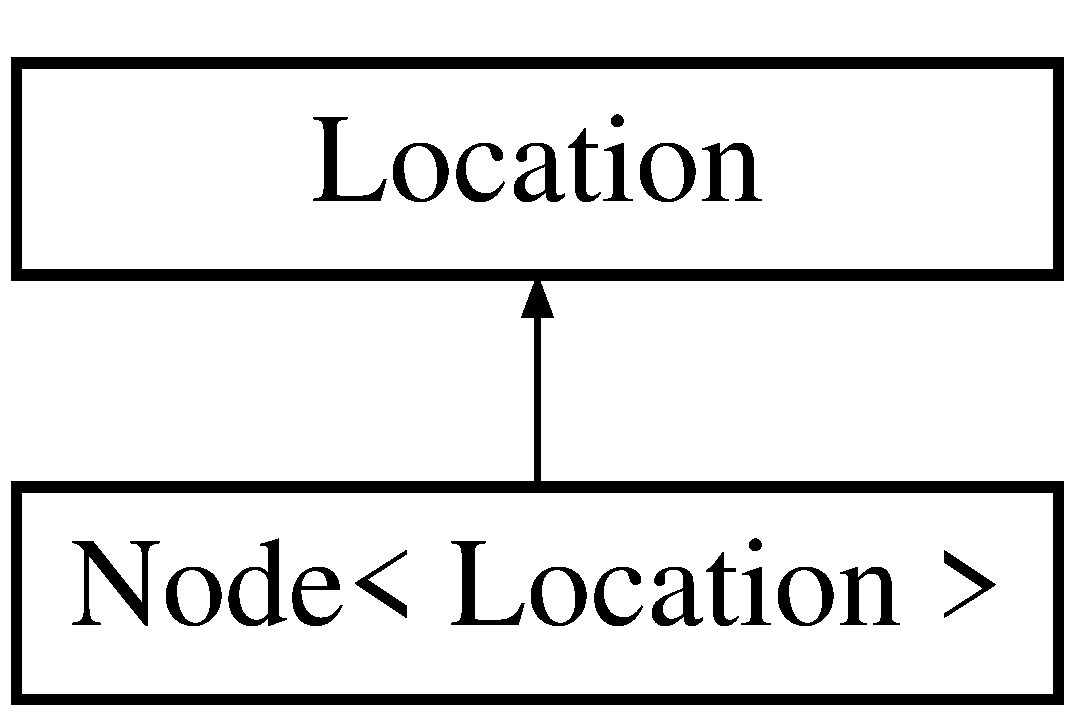
\includegraphics[height=2.000000cm]{classLocation}
\end{center}
\end{figure}
\subsection*{Public Member Functions}
\begin{DoxyCompactItemize}
\item 
\hyperlink{classLocation_a3fc215d3644f4ee28def0cc26dde9637}{Location} (double latitude=0, double longitude=0)
\item 
\hyperlink{classLocation_af5be2c6550bbd96137cbb3144ec3c529}{$\sim$\-Location} ()
\item 
void \hyperlink{classLocation_ae58d423830a2b73d26ee4f0eede072e5}{set\-Start} ()
\item 
bool \hyperlink{classLocation_a585a2e4471c314e177b130f29c0c008e}{start\-Location} ()
\item 
void \hyperlink{classLocation_a05b211d70840608bf0ae10e8981c2eb9}{not\-Start} ()
\item 
double \hyperlink{classLocation_a331ffb113757d06f959655627c96551c}{get\-Long} ()
\item 
double \hyperlink{classLocation_a2ec7b05afffdecadd2f030a3b5144d4c}{get\-Lat} ()
\item 
void \hyperlink{classLocation_afaee021c4f086843afc98f5f8a6883d8}{print\-Coords} ()
\item 
double \hyperlink{classLocation_a5160d825f9dbf4c24d73f87f037ee5a4}{get\-Distance\-To} (\hyperlink{classLocation}{Location} \&loc)
\end{DoxyCompactItemize}
\subsection*{Public Attributes}
\begin{DoxyCompactItemize}
\item 
bool \hyperlink{classLocation_a43b3f7f0d4884faec745edf2ccba621f}{is\-Start}
\item 
int \hyperlink{classLocation_a6be537a226b6add3dac2c3f9f87cdbb9}{location\-I\-D}
\item 
double \hyperlink{classLocation_a7981376ddbae36481fe6058146e1a130}{y}
\item 
double \hyperlink{classLocation_ac794205a47bb99febce79b4c6d614ec1}{x}
\end{DoxyCompactItemize}


\subsection{Constructor \& Destructor Documentation}
\hypertarget{classLocation_a3fc215d3644f4ee28def0cc26dde9637}{\index{Location@{Location}!Location@{Location}}
\index{Location@{Location}!Location@{Location}}
\subsubsection[{Location}]{\setlength{\rightskip}{0pt plus 5cm}Location\-::\-Location (
\begin{DoxyParamCaption}
\item[{double}]{latitude = {\ttfamily 0}, }
\item[{double}]{longitude = {\ttfamily 0}}
\end{DoxyParamCaption}
)}}\label{classLocation_a3fc215d3644f4ee28def0cc26dde9637}
\hypertarget{classLocation_af5be2c6550bbd96137cbb3144ec3c529}{\index{Location@{Location}!$\sim$\-Location@{$\sim$\-Location}}
\index{$\sim$\-Location@{$\sim$\-Location}!Location@{Location}}
\subsubsection[{$\sim$\-Location}]{\setlength{\rightskip}{0pt plus 5cm}Location\-::$\sim$\-Location (
\begin{DoxyParamCaption}
{}
\end{DoxyParamCaption}
)}}\label{classLocation_af5be2c6550bbd96137cbb3144ec3c529}


\subsection{Member Function Documentation}
\hypertarget{classLocation_a5160d825f9dbf4c24d73f87f037ee5a4}{\index{Location@{Location}!get\-Distance\-To@{get\-Distance\-To}}
\index{get\-Distance\-To@{get\-Distance\-To}!Location@{Location}}
\subsubsection[{get\-Distance\-To}]{\setlength{\rightskip}{0pt plus 5cm}double Location\-::get\-Distance\-To (
\begin{DoxyParamCaption}
\item[{{\bf Location} \&}]{loc}
\end{DoxyParamCaption}
)}}\label{classLocation_a5160d825f9dbf4c24d73f87f037ee5a4}
\hypertarget{classLocation_a2ec7b05afffdecadd2f030a3b5144d4c}{\index{Location@{Location}!get\-Lat@{get\-Lat}}
\index{get\-Lat@{get\-Lat}!Location@{Location}}
\subsubsection[{get\-Lat}]{\setlength{\rightskip}{0pt plus 5cm}double Location\-::get\-Lat (
\begin{DoxyParamCaption}
{}
\end{DoxyParamCaption}
)\hspace{0.3cm}{\ttfamily [inline]}}}\label{classLocation_a2ec7b05afffdecadd2f030a3b5144d4c}
\hypertarget{classLocation_a331ffb113757d06f959655627c96551c}{\index{Location@{Location}!get\-Long@{get\-Long}}
\index{get\-Long@{get\-Long}!Location@{Location}}
\subsubsection[{get\-Long}]{\setlength{\rightskip}{0pt plus 5cm}double Location\-::get\-Long (
\begin{DoxyParamCaption}
{}
\end{DoxyParamCaption}
)\hspace{0.3cm}{\ttfamily [inline]}}}\label{classLocation_a331ffb113757d06f959655627c96551c}
\hypertarget{classLocation_a05b211d70840608bf0ae10e8981c2eb9}{\index{Location@{Location}!not\-Start@{not\-Start}}
\index{not\-Start@{not\-Start}!Location@{Location}}
\subsubsection[{not\-Start}]{\setlength{\rightskip}{0pt plus 5cm}void Location\-::not\-Start (
\begin{DoxyParamCaption}
{}
\end{DoxyParamCaption}
)\hspace{0.3cm}{\ttfamily [inline]}}}\label{classLocation_a05b211d70840608bf0ae10e8981c2eb9}
\hypertarget{classLocation_afaee021c4f086843afc98f5f8a6883d8}{\index{Location@{Location}!print\-Coords@{print\-Coords}}
\index{print\-Coords@{print\-Coords}!Location@{Location}}
\subsubsection[{print\-Coords}]{\setlength{\rightskip}{0pt plus 5cm}void Location\-::print\-Coords (
\begin{DoxyParamCaption}
{}
\end{DoxyParamCaption}
)\hspace{0.3cm}{\ttfamily [inline]}}}\label{classLocation_afaee021c4f086843afc98f5f8a6883d8}
\hypertarget{classLocation_ae58d423830a2b73d26ee4f0eede072e5}{\index{Location@{Location}!set\-Start@{set\-Start}}
\index{set\-Start@{set\-Start}!Location@{Location}}
\subsubsection[{set\-Start}]{\setlength{\rightskip}{0pt plus 5cm}void Location\-::set\-Start (
\begin{DoxyParamCaption}
{}
\end{DoxyParamCaption}
)\hspace{0.3cm}{\ttfamily [inline]}}}\label{classLocation_ae58d423830a2b73d26ee4f0eede072e5}
\hypertarget{classLocation_a585a2e4471c314e177b130f29c0c008e}{\index{Location@{Location}!start\-Location@{start\-Location}}
\index{start\-Location@{start\-Location}!Location@{Location}}
\subsubsection[{start\-Location}]{\setlength{\rightskip}{0pt plus 5cm}bool Location\-::start\-Location (
\begin{DoxyParamCaption}
{}
\end{DoxyParamCaption}
)\hspace{0.3cm}{\ttfamily [inline]}}}\label{classLocation_a585a2e4471c314e177b130f29c0c008e}


\subsection{Member Data Documentation}
\hypertarget{classLocation_a43b3f7f0d4884faec745edf2ccba621f}{\index{Location@{Location}!is\-Start@{is\-Start}}
\index{is\-Start@{is\-Start}!Location@{Location}}
\subsubsection[{is\-Start}]{\setlength{\rightskip}{0pt plus 5cm}bool Location\-::is\-Start}}\label{classLocation_a43b3f7f0d4884faec745edf2ccba621f}
\hypertarget{classLocation_a6be537a226b6add3dac2c3f9f87cdbb9}{\index{Location@{Location}!location\-I\-D@{location\-I\-D}}
\index{location\-I\-D@{location\-I\-D}!Location@{Location}}
\subsubsection[{location\-I\-D}]{\setlength{\rightskip}{0pt plus 5cm}int Location\-::location\-I\-D}}\label{classLocation_a6be537a226b6add3dac2c3f9f87cdbb9}
\hypertarget{classLocation_ac794205a47bb99febce79b4c6d614ec1}{\index{Location@{Location}!x@{x}}
\index{x@{x}!Location@{Location}}
\subsubsection[{x}]{\setlength{\rightskip}{0pt plus 5cm}double Location\-::x}}\label{classLocation_ac794205a47bb99febce79b4c6d614ec1}
\hypertarget{classLocation_a7981376ddbae36481fe6058146e1a130}{\index{Location@{Location}!y@{y}}
\index{y@{y}!Location@{Location}}
\subsubsection[{y}]{\setlength{\rightskip}{0pt plus 5cm}double Location\-::y}}\label{classLocation_a7981376ddbae36481fe6058146e1a130}


The documentation for this class was generated from the following files\-:\begin{DoxyCompactItemize}
\item 
Backend/\-Salesman/\hyperlink{Location_8h}{Location.\-h}\item 
Backend/\-Salesman/\hyperlink{Location_8cpp}{Location.\-cpp}\end{DoxyCompactItemize}

\hypertarget{classMatrix}{\section{Matrix Class Reference}
\label{classMatrix}\index{Matrix@{Matrix}}
}


{\ttfamily \#include \char`\"{}Matrices.\-h\char`\"{}}

\subsection*{Public Member Functions}
\begin{DoxyCompactItemize}
\item 
\hyperlink{classMatrix_a6c846d0a46676ff6addbcd04e2d516cc}{Matrix} (int elements)
\item 
\hyperlink{classMatrix_a9b1c3627f573d78a2f08623fdfef990f}{$\sim$\-Matrix} ()
\item 
bool \hyperlink{classMatrix_a98ba0c156a03a068759c4c2b8eb837eb}{set\-Element} (int row, int column, double value)
\item 
double \hyperlink{classMatrix_a37b3a00db12f5838c164960ecf2ce42e}{get\-Element} (int row, int column)
\item 
void \hyperlink{classMatrix_ad5fe18fa5ffe97bda044000d45bf1547}{show\-Matrix} ()
\item 
int \hyperlink{classMatrix_af4421f66ac5f486116ebfe10f2cced18}{number\-Of\-Columns} ()
\end{DoxyCompactItemize}
\subsection*{Private Attributes}
\begin{DoxyCompactItemize}
\item 
double $\ast$ \hyperlink{classMatrix_a19505b0b139553ad1ee2291f3d8385a9}{values}
\item 
int \hyperlink{classMatrix_afd4ab1ffa8fadfcaae4ebcf7802c0fef}{number\-\_\-of\-\_\-columns}
\item 
int \hyperlink{classMatrix_ad88772bca79eec502f3737b027431c60}{number\-\_\-of\-\_\-elements}
\end{DoxyCompactItemize}


\subsection{Constructor \& Destructor Documentation}
\hypertarget{classMatrix_a6c846d0a46676ff6addbcd04e2d516cc}{\index{Matrix@{Matrix}!Matrix@{Matrix}}
\index{Matrix@{Matrix}!Matrix@{Matrix}}
\subsubsection[{Matrix}]{\setlength{\rightskip}{0pt plus 5cm}Matrix\-::\-Matrix (
\begin{DoxyParamCaption}
\item[{int}]{elements}
\end{DoxyParamCaption}
)}}\label{classMatrix_a6c846d0a46676ff6addbcd04e2d516cc}
\hypertarget{classMatrix_a9b1c3627f573d78a2f08623fdfef990f}{\index{Matrix@{Matrix}!$\sim$\-Matrix@{$\sim$\-Matrix}}
\index{$\sim$\-Matrix@{$\sim$\-Matrix}!Matrix@{Matrix}}
\subsubsection[{$\sim$\-Matrix}]{\setlength{\rightskip}{0pt plus 5cm}Matrix\-::$\sim$\-Matrix (
\begin{DoxyParamCaption}
{}
\end{DoxyParamCaption}
)}}\label{classMatrix_a9b1c3627f573d78a2f08623fdfef990f}


\subsection{Member Function Documentation}
\hypertarget{classMatrix_a37b3a00db12f5838c164960ecf2ce42e}{\index{Matrix@{Matrix}!get\-Element@{get\-Element}}
\index{get\-Element@{get\-Element}!Matrix@{Matrix}}
\subsubsection[{get\-Element}]{\setlength{\rightskip}{0pt plus 5cm}double Matrix\-::get\-Element (
\begin{DoxyParamCaption}
\item[{int}]{row, }
\item[{int}]{column}
\end{DoxyParamCaption}
)}}\label{classMatrix_a37b3a00db12f5838c164960ecf2ce42e}
\hypertarget{classMatrix_af4421f66ac5f486116ebfe10f2cced18}{\index{Matrix@{Matrix}!number\-Of\-Columns@{number\-Of\-Columns}}
\index{number\-Of\-Columns@{number\-Of\-Columns}!Matrix@{Matrix}}
\subsubsection[{number\-Of\-Columns}]{\setlength{\rightskip}{0pt plus 5cm}int Matrix\-::number\-Of\-Columns (
\begin{DoxyParamCaption}
{}
\end{DoxyParamCaption}
)\hspace{0.3cm}{\ttfamily [inline]}}}\label{classMatrix_af4421f66ac5f486116ebfe10f2cced18}
\hypertarget{classMatrix_a98ba0c156a03a068759c4c2b8eb837eb}{\index{Matrix@{Matrix}!set\-Element@{set\-Element}}
\index{set\-Element@{set\-Element}!Matrix@{Matrix}}
\subsubsection[{set\-Element}]{\setlength{\rightskip}{0pt plus 5cm}bool Matrix\-::set\-Element (
\begin{DoxyParamCaption}
\item[{int}]{row, }
\item[{int}]{column, }
\item[{double}]{value}
\end{DoxyParamCaption}
)}}\label{classMatrix_a98ba0c156a03a068759c4c2b8eb837eb}
\hypertarget{classMatrix_ad5fe18fa5ffe97bda044000d45bf1547}{\index{Matrix@{Matrix}!show\-Matrix@{show\-Matrix}}
\index{show\-Matrix@{show\-Matrix}!Matrix@{Matrix}}
\subsubsection[{show\-Matrix}]{\setlength{\rightskip}{0pt plus 5cm}void Matrix\-::show\-Matrix (
\begin{DoxyParamCaption}
{}
\end{DoxyParamCaption}
)}}\label{classMatrix_ad5fe18fa5ffe97bda044000d45bf1547}


\subsection{Member Data Documentation}
\hypertarget{classMatrix_afd4ab1ffa8fadfcaae4ebcf7802c0fef}{\index{Matrix@{Matrix}!number\-\_\-of\-\_\-columns@{number\-\_\-of\-\_\-columns}}
\index{number\-\_\-of\-\_\-columns@{number\-\_\-of\-\_\-columns}!Matrix@{Matrix}}
\subsubsection[{number\-\_\-of\-\_\-columns}]{\setlength{\rightskip}{0pt plus 5cm}int Matrix\-::number\-\_\-of\-\_\-columns\hspace{0.3cm}{\ttfamily [private]}}}\label{classMatrix_afd4ab1ffa8fadfcaae4ebcf7802c0fef}
\hypertarget{classMatrix_ad88772bca79eec502f3737b027431c60}{\index{Matrix@{Matrix}!number\-\_\-of\-\_\-elements@{number\-\_\-of\-\_\-elements}}
\index{number\-\_\-of\-\_\-elements@{number\-\_\-of\-\_\-elements}!Matrix@{Matrix}}
\subsubsection[{number\-\_\-of\-\_\-elements}]{\setlength{\rightskip}{0pt plus 5cm}int Matrix\-::number\-\_\-of\-\_\-elements\hspace{0.3cm}{\ttfamily [private]}}}\label{classMatrix_ad88772bca79eec502f3737b027431c60}
\hypertarget{classMatrix_a19505b0b139553ad1ee2291f3d8385a9}{\index{Matrix@{Matrix}!values@{values}}
\index{values@{values}!Matrix@{Matrix}}
\subsubsection[{values}]{\setlength{\rightskip}{0pt plus 5cm}double$\ast$ Matrix\-::values\hspace{0.3cm}{\ttfamily [private]}}}\label{classMatrix_a19505b0b139553ad1ee2291f3d8385a9}


The documentation for this class was generated from the following files\-:\begin{DoxyCompactItemize}
\item 
tools/\hyperlink{Matrices_8h}{Matrices.\-h}\item 
tools/\hyperlink{Matrices_8cpp}{Matrices.\-cpp}\end{DoxyCompactItemize}

\hypertarget{classNode}{\section{Node$<$ Type $>$ Class Template Reference}
\label{classNode}\index{Node$<$ Type $>$@{Node$<$ Type $>$}}
}


{\ttfamily \#include \char`\"{}Linked\-List.\-h\char`\"{}}

Inheritance diagram for Node$<$ Type $>$\-:\begin{figure}[H]
\begin{center}
\leavevmode
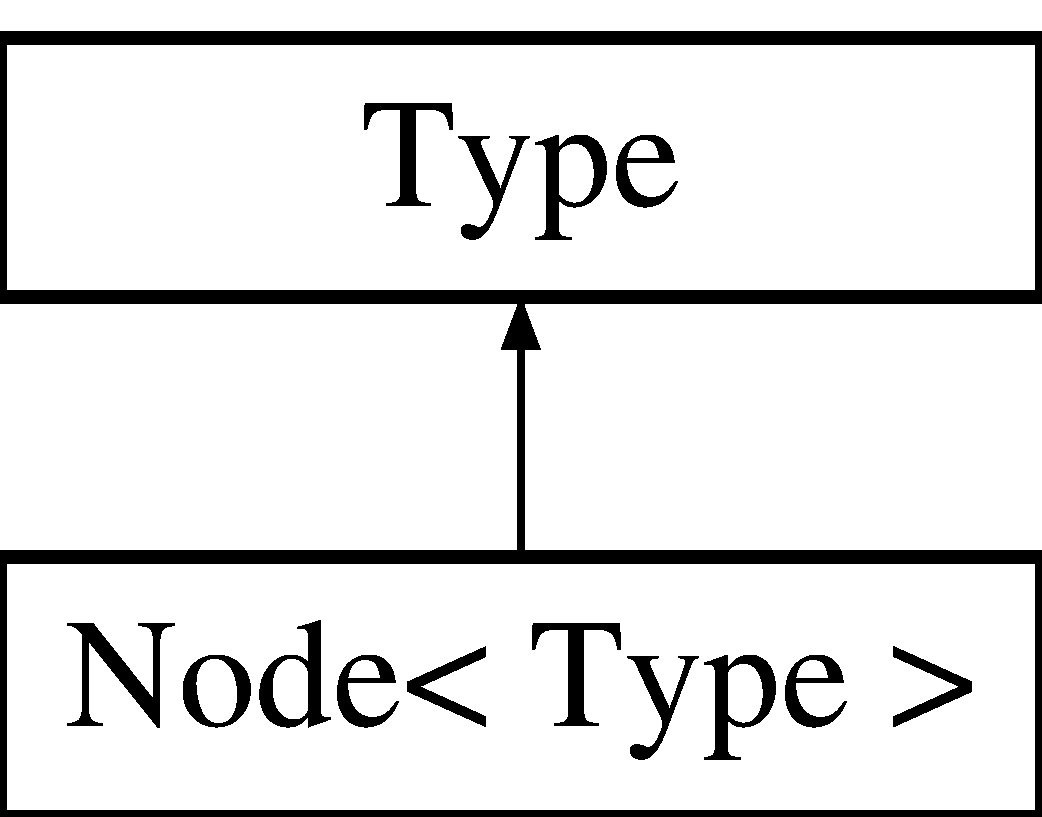
\includegraphics[height=2.000000cm]{classNode}
\end{center}
\end{figure}
\subsection*{Public Member Functions}
\begin{DoxyCompactItemize}
\item 
\hyperlink{classNode_a42a737af32efbba6e1fd950f7aca8af8}{Node} (double latitude, double longitude)
\end{DoxyCompactItemize}
\subsection*{Public Attributes}
\begin{DoxyCompactItemize}
\item 
\hyperlink{classNode}{Node}$<$ Type $>$ $\ast$ \hyperlink{classNode_ac3eee180a74bd4af7fbcf7d071bfae4f}{next}
\item 
\hyperlink{classNode}{Node}$<$ Type $>$ $\ast$ \hyperlink{classNode_a3b482296542a8c0106ca107d189648e7}{previous}
\end{DoxyCompactItemize}


\subsection{Constructor \& Destructor Documentation}
\hypertarget{classNode_a42a737af32efbba6e1fd950f7aca8af8}{\index{Node@{Node}!Node@{Node}}
\index{Node@{Node}!Node@{Node}}
\subsubsection[{Node}]{\setlength{\rightskip}{0pt plus 5cm}template$<$class Type$>$ {\bf Node}$<$ Type $>$\-::{\bf Node} (
\begin{DoxyParamCaption}
\item[{double}]{latitude, }
\item[{double}]{longitude}
\end{DoxyParamCaption}
)\hspace{0.3cm}{\ttfamily [inline]}}}\label{classNode_a42a737af32efbba6e1fd950f7aca8af8}


\subsection{Member Data Documentation}
\hypertarget{classNode_ac3eee180a74bd4af7fbcf7d071bfae4f}{\index{Node@{Node}!next@{next}}
\index{next@{next}!Node@{Node}}
\subsubsection[{next}]{\setlength{\rightskip}{0pt plus 5cm}template$<$class Type$>$ {\bf Node}$<$Type$>$$\ast$ {\bf Node}$<$ Type $>$\-::next}}\label{classNode_ac3eee180a74bd4af7fbcf7d071bfae4f}
\hypertarget{classNode_a3b482296542a8c0106ca107d189648e7}{\index{Node@{Node}!previous@{previous}}
\index{previous@{previous}!Node@{Node}}
\subsubsection[{previous}]{\setlength{\rightskip}{0pt plus 5cm}template$<$class Type$>$ {\bf Node}$<$Type$>$$\ast$ {\bf Node}$<$ Type $>$\-::previous}}\label{classNode_a3b482296542a8c0106ca107d189648e7}


The documentation for this class was generated from the following file\-:\begin{DoxyCompactItemize}
\item 
tools/\hyperlink{LinkedList_8h}{Linked\-List.\-h}\end{DoxyCompactItemize}

\hypertarget{classPyFunc}{\section{Py\-Func$<$ Type $>$ Class Template Reference}
\label{classPyFunc}\index{Py\-Func$<$ Type $>$@{Py\-Func$<$ Type $>$}}
}


{\ttfamily \#include \char`\"{}Py\-Func.\-h\char`\"{}}

Inheritance diagram for Py\-Func$<$ Type $>$\-:\begin{figure}[H]
\begin{center}
\leavevmode
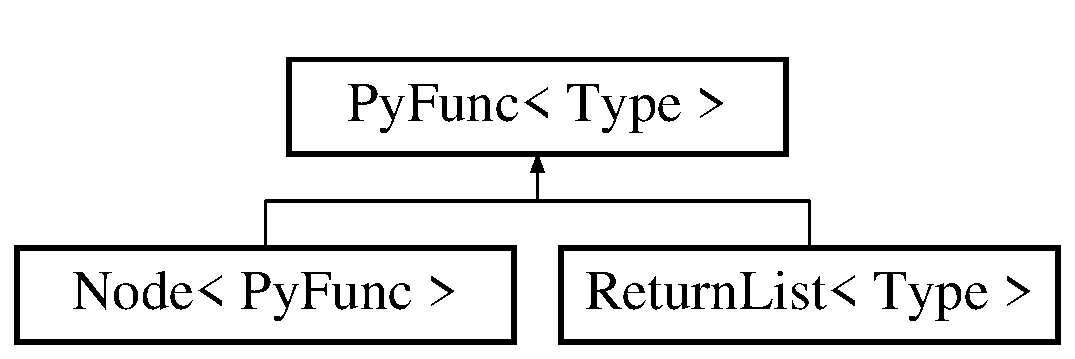
\includegraphics[height=2.000000cm]{classPyFunc}
\end{center}
\end{figure}
\subsection*{Public Member Functions}
\begin{DoxyCompactItemize}
\item 
\hyperlink{classPyFunc_abdf959abaa390e591d6831631a63b847}{Py\-Func} (const char $\ast$Module, const char $\ast$Func\-Name, char $\ast$File\-Name)
\item 
\hyperlink{classPyFunc_a5813fdcef05c12cb8cc6049386ca4509}{$\sim$\-Py\-Func} ()
\item 
bool \hyperlink{classPyFunc_a9765fda4c500e4225a2d5a766fd4d13b}{valid\-Func} ()
\end{DoxyCompactItemize}
\subsection*{Protected Attributes}
\begin{DoxyCompactItemize}
\item 
Py\-Object $\ast$ \hyperlink{classPyFunc_aa87d68b9046b473e3cfeb4a0e08dccf0}{p\-Module}
\item 
Py\-Object $\ast$ \hyperlink{classPyFunc_aee7f0c1f281e63e0d26ff71b9868c086}{p\-Name}
\item 
Py\-Object $\ast$ \hyperlink{classPyFunc_a941eb18b7d22632c55b41652d79b0481}{p\-Func}
\item 
Py\-Object $\ast$ \hyperlink{classPyFunc_af3d520a4b2580b0ac96ad5ee9f745335}{p\-List}
\item 
Py\-Object $\ast$ \hyperlink{classPyFunc_a3c63064658876c190224c4adc5f5dc07}{p\-Value}
\item 
Py\-Object $\ast$ \hyperlink{classPyFunc_a9794285af7ee57f561e56685b374ff63}{p\-List\-Length}
\item 
Py\-Object \hyperlink{classPyFunc_afcc6a33961a461a500f5ea5b9d280e3e}{p\-List\-Item}
\item 
bool \hyperlink{classPyFunc_a6b9334f10ee479b14189e2bb7d9d4cc3}{is\-Valid}
\end{DoxyCompactItemize}


\subsection{Constructor \& Destructor Documentation}
\hypertarget{classPyFunc_abdf959abaa390e591d6831631a63b847}{\index{Py\-Func@{Py\-Func}!Py\-Func@{Py\-Func}}
\index{Py\-Func@{Py\-Func}!PyFunc@{Py\-Func}}
\subsubsection[{Py\-Func}]{\setlength{\rightskip}{0pt plus 5cm}template$<$class Type $>$ {\bf Py\-Func}$<$ Type $>$\-::{\bf Py\-Func} (
\begin{DoxyParamCaption}
\item[{const char $\ast$}]{Module, }
\item[{const char $\ast$}]{Func\-Name, }
\item[{char $\ast$}]{File\-Name}
\end{DoxyParamCaption}
)}}\label{classPyFunc_abdf959abaa390e591d6831631a63b847}
\hypertarget{classPyFunc_a5813fdcef05c12cb8cc6049386ca4509}{\index{Py\-Func@{Py\-Func}!$\sim$\-Py\-Func@{$\sim$\-Py\-Func}}
\index{$\sim$\-Py\-Func@{$\sim$\-Py\-Func}!PyFunc@{Py\-Func}}
\subsubsection[{$\sim$\-Py\-Func}]{\setlength{\rightskip}{0pt plus 5cm}template$<$class Type $>$ {\bf Py\-Func}$<$ Type $>$\-::$\sim${\bf Py\-Func} (
\begin{DoxyParamCaption}
{}
\end{DoxyParamCaption}
)}}\label{classPyFunc_a5813fdcef05c12cb8cc6049386ca4509}


\subsection{Member Function Documentation}
\hypertarget{classPyFunc_a9765fda4c500e4225a2d5a766fd4d13b}{\index{Py\-Func@{Py\-Func}!valid\-Func@{valid\-Func}}
\index{valid\-Func@{valid\-Func}!PyFunc@{Py\-Func}}
\subsubsection[{valid\-Func}]{\setlength{\rightskip}{0pt plus 5cm}template$<$class Type $>$ bool {\bf Py\-Func}$<$ Type $>$\-::valid\-Func (
\begin{DoxyParamCaption}
{}
\end{DoxyParamCaption}
)\hspace{0.3cm}{\ttfamily [inline]}}}\label{classPyFunc_a9765fda4c500e4225a2d5a766fd4d13b}


\subsection{Member Data Documentation}
\hypertarget{classPyFunc_a6b9334f10ee479b14189e2bb7d9d4cc3}{\index{Py\-Func@{Py\-Func}!is\-Valid@{is\-Valid}}
\index{is\-Valid@{is\-Valid}!PyFunc@{Py\-Func}}
\subsubsection[{is\-Valid}]{\setlength{\rightskip}{0pt plus 5cm}template$<$class Type $>$ bool {\bf Py\-Func}$<$ Type $>$\-::is\-Valid\hspace{0.3cm}{\ttfamily [protected]}}}\label{classPyFunc_a6b9334f10ee479b14189e2bb7d9d4cc3}
\hypertarget{classPyFunc_a941eb18b7d22632c55b41652d79b0481}{\index{Py\-Func@{Py\-Func}!p\-Func@{p\-Func}}
\index{p\-Func@{p\-Func}!PyFunc@{Py\-Func}}
\subsubsection[{p\-Func}]{\setlength{\rightskip}{0pt plus 5cm}template$<$class Type $>$ Py\-Object $\ast$ {\bf Py\-Func}$<$ Type $>$\-::p\-Func\hspace{0.3cm}{\ttfamily [protected]}}}\label{classPyFunc_a941eb18b7d22632c55b41652d79b0481}
\hypertarget{classPyFunc_af3d520a4b2580b0ac96ad5ee9f745335}{\index{Py\-Func@{Py\-Func}!p\-List@{p\-List}}
\index{p\-List@{p\-List}!PyFunc@{Py\-Func}}
\subsubsection[{p\-List}]{\setlength{\rightskip}{0pt plus 5cm}template$<$class Type $>$ Py\-Object $\ast$ {\bf Py\-Func}$<$ Type $>$\-::p\-List\hspace{0.3cm}{\ttfamily [protected]}}}\label{classPyFunc_af3d520a4b2580b0ac96ad5ee9f745335}
\hypertarget{classPyFunc_afcc6a33961a461a500f5ea5b9d280e3e}{\index{Py\-Func@{Py\-Func}!p\-List\-Item@{p\-List\-Item}}
\index{p\-List\-Item@{p\-List\-Item}!PyFunc@{Py\-Func}}
\subsubsection[{p\-List\-Item}]{\setlength{\rightskip}{0pt plus 5cm}template$<$class Type $>$ Py\-Object {\bf Py\-Func}$<$ Type $>$\-::p\-List\-Item\hspace{0.3cm}{\ttfamily [protected]}}}\label{classPyFunc_afcc6a33961a461a500f5ea5b9d280e3e}
\hypertarget{classPyFunc_a9794285af7ee57f561e56685b374ff63}{\index{Py\-Func@{Py\-Func}!p\-List\-Length@{p\-List\-Length}}
\index{p\-List\-Length@{p\-List\-Length}!PyFunc@{Py\-Func}}
\subsubsection[{p\-List\-Length}]{\setlength{\rightskip}{0pt plus 5cm}template$<$class Type $>$ Py\-Object$\ast$ {\bf Py\-Func}$<$ Type $>$\-::p\-List\-Length\hspace{0.3cm}{\ttfamily [protected]}}}\label{classPyFunc_a9794285af7ee57f561e56685b374ff63}
\hypertarget{classPyFunc_aa87d68b9046b473e3cfeb4a0e08dccf0}{\index{Py\-Func@{Py\-Func}!p\-Module@{p\-Module}}
\index{p\-Module@{p\-Module}!PyFunc@{Py\-Func}}
\subsubsection[{p\-Module}]{\setlength{\rightskip}{0pt plus 5cm}template$<$class Type $>$ Py\-Object$\ast$ {\bf Py\-Func}$<$ Type $>$\-::p\-Module\hspace{0.3cm}{\ttfamily [protected]}}}\label{classPyFunc_aa87d68b9046b473e3cfeb4a0e08dccf0}
\hypertarget{classPyFunc_aee7f0c1f281e63e0d26ff71b9868c086}{\index{Py\-Func@{Py\-Func}!p\-Name@{p\-Name}}
\index{p\-Name@{p\-Name}!PyFunc@{Py\-Func}}
\subsubsection[{p\-Name}]{\setlength{\rightskip}{0pt plus 5cm}template$<$class Type $>$ Py\-Object $\ast$ {\bf Py\-Func}$<$ Type $>$\-::p\-Name\hspace{0.3cm}{\ttfamily [protected]}}}\label{classPyFunc_aee7f0c1f281e63e0d26ff71b9868c086}
\hypertarget{classPyFunc_a3c63064658876c190224c4adc5f5dc07}{\index{Py\-Func@{Py\-Func}!p\-Value@{p\-Value}}
\index{p\-Value@{p\-Value}!PyFunc@{Py\-Func}}
\subsubsection[{p\-Value}]{\setlength{\rightskip}{0pt plus 5cm}template$<$class Type $>$ Py\-Object $\ast$ {\bf Py\-Func}$<$ Type $>$\-::p\-Value\hspace{0.3cm}{\ttfamily [protected]}}}\label{classPyFunc_a3c63064658876c190224c4adc5f5dc07}


The documentation for this class was generated from the following files\-:\begin{DoxyCompactItemize}
\item 
tools/\-Python/\hyperlink{PyFunc_8h}{Py\-Func.\-h}\item 
tools/\-Python/\hyperlink{_8PyFunc_8cpp}{.\-Py\-Func.\-cpp}\end{DoxyCompactItemize}

\hypertarget{classPyI}{\section{Py\-I Class Reference}
\label{classPyI}\index{Py\-I@{Py\-I}}
}


{\ttfamily \#include \char`\"{}.\-Py\-I.\-h\char`\"{}}

\subsection*{Public Member Functions}
\begin{DoxyCompactItemize}
\item 
\hyperlink{classPyI_a40095536c9eeb4e315c1366839545af3}{Py\-I} ()
\item 
\hyperlink{classPyI_ae3f36823af7e166896217875450de15c}{$\sim$\-Py\-I} ()
\item 
void \hyperlink{classPyI_adc3abd8506cdce16756c2c691f14ede7}{add\-Function} (\hyperlink{classPyFunc}{Py\-Func} $\ast$p\-Func)
\end{DoxyCompactItemize}
\subsection*{Private Attributes}
\begin{DoxyCompactItemize}
\item 
\hyperlink{classLinkedList}{Linked\-List}$<$ \hyperlink{classPyFunc}{Py\-Func} $>$ $\ast$ \hyperlink{classPyI_a304ad7cd3869d2281e35113c2d893192}{func\-List}
\end{DoxyCompactItemize}


\subsection{Constructor \& Destructor Documentation}
\hypertarget{classPyI_a40095536c9eeb4e315c1366839545af3}{\index{Py\-I@{Py\-I}!Py\-I@{Py\-I}}
\index{Py\-I@{Py\-I}!PyI@{Py\-I}}
\subsubsection[{Py\-I}]{\setlength{\rightskip}{0pt plus 5cm}Py\-I\-::\-Py\-I (
\begin{DoxyParamCaption}
{}
\end{DoxyParamCaption}
)}}\label{classPyI_a40095536c9eeb4e315c1366839545af3}
\hypertarget{classPyI_ae3f36823af7e166896217875450de15c}{\index{Py\-I@{Py\-I}!$\sim$\-Py\-I@{$\sim$\-Py\-I}}
\index{$\sim$\-Py\-I@{$\sim$\-Py\-I}!PyI@{Py\-I}}
\subsubsection[{$\sim$\-Py\-I}]{\setlength{\rightskip}{0pt plus 5cm}Py\-I\-::$\sim$\-Py\-I (
\begin{DoxyParamCaption}
{}
\end{DoxyParamCaption}
)}}\label{classPyI_ae3f36823af7e166896217875450de15c}


\subsection{Member Function Documentation}
\hypertarget{classPyI_adc3abd8506cdce16756c2c691f14ede7}{\index{Py\-I@{Py\-I}!add\-Function@{add\-Function}}
\index{add\-Function@{add\-Function}!PyI@{Py\-I}}
\subsubsection[{add\-Function}]{\setlength{\rightskip}{0pt plus 5cm}void Py\-I\-::add\-Function (
\begin{DoxyParamCaption}
\item[{{\bf Py\-Func} $\ast$}]{p\-Func}
\end{DoxyParamCaption}
)}}\label{classPyI_adc3abd8506cdce16756c2c691f14ede7}


\subsection{Member Data Documentation}
\hypertarget{classPyI_a304ad7cd3869d2281e35113c2d893192}{\index{Py\-I@{Py\-I}!func\-List@{func\-List}}
\index{func\-List@{func\-List}!PyI@{Py\-I}}
\subsubsection[{func\-List}]{\setlength{\rightskip}{0pt plus 5cm}{\bf Linked\-List}$<${\bf Py\-Func}$>$$\ast$ Py\-I\-::func\-List\hspace{0.3cm}{\ttfamily [private]}}}\label{classPyI_a304ad7cd3869d2281e35113c2d893192}


The documentation for this class was generated from the following files\-:\begin{DoxyCompactItemize}
\item 
tools/\-Python/\hyperlink{_8PyI_8h}{.\-Py\-I.\-h}\item 
tools/\-Python/\hyperlink{_8PyI_8cpp}{.\-Py\-I.\-cpp}\end{DoxyCompactItemize}

\hypertarget{classReturnList}{\section{Return\-List$<$ Type $>$ Class Template Reference}
\label{classReturnList}\index{Return\-List$<$ Type $>$@{Return\-List$<$ Type $>$}}
}


{\ttfamily \#include \char`\"{}Functions.\-h\char`\"{}}

Inheritance diagram for Return\-List$<$ Type $>$\-:\begin{figure}[H]
\begin{center}
\leavevmode
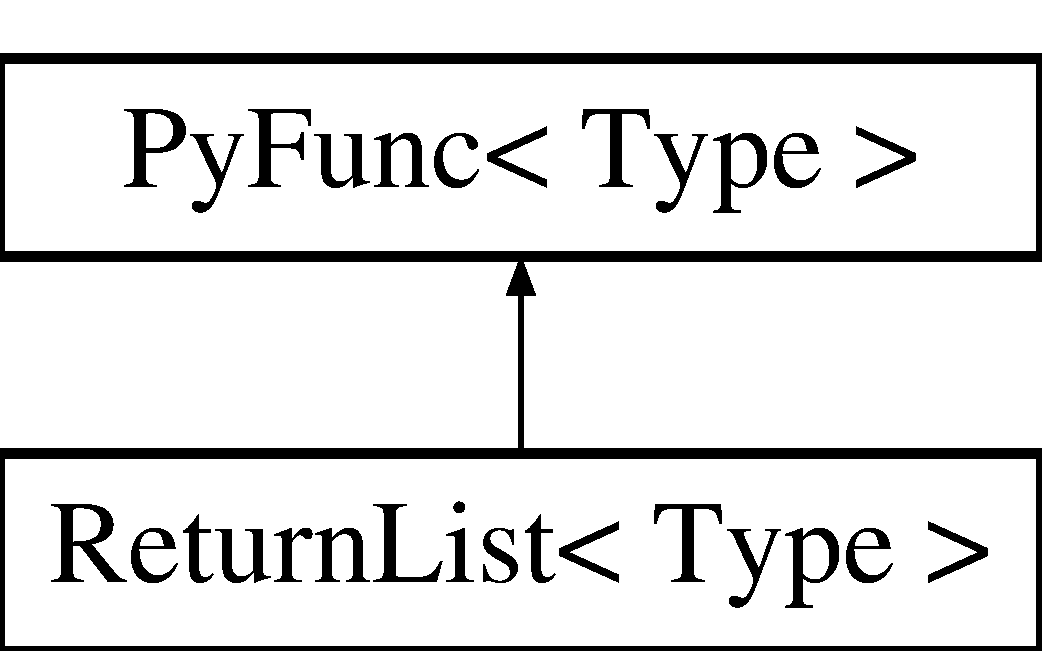
\includegraphics[height=2.000000cm]{classReturnList}
\end{center}
\end{figure}
\subsection*{Public Member Functions}
\begin{DoxyCompactItemize}
\item 
\hyperlink{classReturnList_a30a2da53557b38441e1a5b992788a1ad}{Return\-List} (const char $\ast$Module\-Name, const char $\ast$Func\-Name, char $\ast$File\-Name)
\item 
Type $\ast$ \hyperlink{classReturnList_ae95ced17d74728e7c27b684f14d57706}{call\-Function} ()
\end{DoxyCompactItemize}
\subsection*{Additional Inherited Members}


\subsection{Constructor \& Destructor Documentation}
\hypertarget{classReturnList_a30a2da53557b38441e1a5b992788a1ad}{\index{Return\-List@{Return\-List}!Return\-List@{Return\-List}}
\index{Return\-List@{Return\-List}!ReturnList@{Return\-List}}
\subsubsection[{Return\-List}]{\setlength{\rightskip}{0pt plus 5cm}template$<$class Type $>$ {\bf Return\-List}$<$ Type $>$\-::{\bf Return\-List} (
\begin{DoxyParamCaption}
\item[{const char $\ast$}]{Module\-Name, }
\item[{const char $\ast$}]{Func\-Name, }
\item[{char $\ast$}]{File\-Name}
\end{DoxyParamCaption}
)\hspace{0.3cm}{\ttfamily [inline]}}}\label{classReturnList_a30a2da53557b38441e1a5b992788a1ad}


\subsection{Member Function Documentation}
\hypertarget{classReturnList_ae95ced17d74728e7c27b684f14d57706}{\index{Return\-List@{Return\-List}!call\-Function@{call\-Function}}
\index{call\-Function@{call\-Function}!ReturnList@{Return\-List}}
\subsubsection[{call\-Function}]{\setlength{\rightskip}{0pt plus 5cm}template$<$class Type $>$ Type $\ast$ {\bf Return\-List}$<$ Type $>$\-::call\-Function (
\begin{DoxyParamCaption}
{}
\end{DoxyParamCaption}
)}}\label{classReturnList_ae95ced17d74728e7c27b684f14d57706}


The documentation for this class was generated from the following files\-:\begin{DoxyCompactItemize}
\item 
tools/\-Python/\hyperlink{Functions_8h}{Functions.\-h}\item 
tools/\-Python/\hyperlink{_8Functions_8cpp}{.\-Functions.\-cpp}\end{DoxyCompactItemize}

\hypertarget{classSalesman}{\section{Salesman Class Reference}
\label{classSalesman}\index{Salesman@{Salesman}}
}


{\ttfamily \#include \char`\"{}Salesman.\-h\char`\"{}}

\subsection*{Public Member Functions}
\begin{DoxyCompactItemize}
\item 
\hyperlink{classSalesman_ab32efbb2c7f7d57dbdcf9575370d1bce}{Salesman} ()
\item 
\hyperlink{classSalesman_af8e121d27b685f74edd1b8bc2964a668}{$\sim$\-Salesman} ()
\item 
void \hyperlink{classSalesman_a395e4d58d2c215370ec462fbf88d9db6}{add\-Location} (double longitude, double latitude)
\item 
void \hyperlink{classSalesman_adfdb2c81bbebdfa1415ff0955d63abdc}{show\-Locations} ()
\item 
void \hyperlink{classSalesman_a0d58b5de2bd9befcacd085fe930166ad}{show\-Route} ()
\item 
bool \hyperlink{classSalesman_a1590194b6a0e1edd9b7a156e00e5844e}{populate\-Matrix} ()
\item 
void \hyperlink{classSalesman_a4221f3823416c5a7b44cef13fce58700}{calculate\-Route} ()
\end{DoxyCompactItemize}
\subsection*{Private Attributes}
\begin{DoxyCompactItemize}
\item 
\hyperlink{classLinkedList}{Linked\-List}$<$ \hyperlink{classLocation}{Location} $>$ $\ast$ \hyperlink{classSalesman_ab9e104c49e0f5ac61deebb86520b229b}{locations}
\item 
\hyperlink{classLinkedList}{Linked\-List}$<$ \hyperlink{classLocation}{Location} $>$ $\ast$ \hyperlink{classSalesman_a7e6c1099741dd8cfc6d44784b026eb44}{route}
\item 
\hyperlink{classMatrix}{Matrix} $\ast$ \hyperlink{classSalesman_a11e52f4aa2750626800eecf2201c9088}{distance\-Matrix}
\item 
bool \hyperlink{classSalesman_abb3c72fd5efc1fb172d3271f82811053}{has\-Matrix}
\end{DoxyCompactItemize}


\subsection{Constructor \& Destructor Documentation}
\hypertarget{classSalesman_ab32efbb2c7f7d57dbdcf9575370d1bce}{\index{Salesman@{Salesman}!Salesman@{Salesman}}
\index{Salesman@{Salesman}!Salesman@{Salesman}}
\subsubsection[{Salesman}]{\setlength{\rightskip}{0pt plus 5cm}Salesman\-::\-Salesman (
\begin{DoxyParamCaption}
{}
\end{DoxyParamCaption}
)}}\label{classSalesman_ab32efbb2c7f7d57dbdcf9575370d1bce}
\hypertarget{classSalesman_af8e121d27b685f74edd1b8bc2964a668}{\index{Salesman@{Salesman}!$\sim$\-Salesman@{$\sim$\-Salesman}}
\index{$\sim$\-Salesman@{$\sim$\-Salesman}!Salesman@{Salesman}}
\subsubsection[{$\sim$\-Salesman}]{\setlength{\rightskip}{0pt plus 5cm}Salesman\-::$\sim$\-Salesman (
\begin{DoxyParamCaption}
{}
\end{DoxyParamCaption}
)}}\label{classSalesman_af8e121d27b685f74edd1b8bc2964a668}


\subsection{Member Function Documentation}
\hypertarget{classSalesman_a395e4d58d2c215370ec462fbf88d9db6}{\index{Salesman@{Salesman}!add\-Location@{add\-Location}}
\index{add\-Location@{add\-Location}!Salesman@{Salesman}}
\subsubsection[{add\-Location}]{\setlength{\rightskip}{0pt plus 5cm}void Salesman\-::add\-Location (
\begin{DoxyParamCaption}
\item[{double}]{longitude, }
\item[{double}]{latitude}
\end{DoxyParamCaption}
)}}\label{classSalesman_a395e4d58d2c215370ec462fbf88d9db6}
\hypertarget{classSalesman_a4221f3823416c5a7b44cef13fce58700}{\index{Salesman@{Salesman}!calculate\-Route@{calculate\-Route}}
\index{calculate\-Route@{calculate\-Route}!Salesman@{Salesman}}
\subsubsection[{calculate\-Route}]{\setlength{\rightskip}{0pt plus 5cm}void Salesman\-::calculate\-Route (
\begin{DoxyParamCaption}
{}
\end{DoxyParamCaption}
)}}\label{classSalesman_a4221f3823416c5a7b44cef13fce58700}
\hypertarget{classSalesman_a1590194b6a0e1edd9b7a156e00e5844e}{\index{Salesman@{Salesman}!populate\-Matrix@{populate\-Matrix}}
\index{populate\-Matrix@{populate\-Matrix}!Salesman@{Salesman}}
\subsubsection[{populate\-Matrix}]{\setlength{\rightskip}{0pt plus 5cm}bool Salesman\-::populate\-Matrix (
\begin{DoxyParamCaption}
{}
\end{DoxyParamCaption}
)}}\label{classSalesman_a1590194b6a0e1edd9b7a156e00e5844e}
\hypertarget{classSalesman_adfdb2c81bbebdfa1415ff0955d63abdc}{\index{Salesman@{Salesman}!show\-Locations@{show\-Locations}}
\index{show\-Locations@{show\-Locations}!Salesman@{Salesman}}
\subsubsection[{show\-Locations}]{\setlength{\rightskip}{0pt plus 5cm}void Salesman\-::show\-Locations (
\begin{DoxyParamCaption}
{}
\end{DoxyParamCaption}
)}}\label{classSalesman_adfdb2c81bbebdfa1415ff0955d63abdc}
\hypertarget{classSalesman_a0d58b5de2bd9befcacd085fe930166ad}{\index{Salesman@{Salesman}!show\-Route@{show\-Route}}
\index{show\-Route@{show\-Route}!Salesman@{Salesman}}
\subsubsection[{show\-Route}]{\setlength{\rightskip}{0pt plus 5cm}void Salesman\-::show\-Route (
\begin{DoxyParamCaption}
{}
\end{DoxyParamCaption}
)}}\label{classSalesman_a0d58b5de2bd9befcacd085fe930166ad}


\subsection{Member Data Documentation}
\hypertarget{classSalesman_a11e52f4aa2750626800eecf2201c9088}{\index{Salesman@{Salesman}!distance\-Matrix@{distance\-Matrix}}
\index{distance\-Matrix@{distance\-Matrix}!Salesman@{Salesman}}
\subsubsection[{distance\-Matrix}]{\setlength{\rightskip}{0pt plus 5cm}{\bf Matrix}$\ast$ Salesman\-::distance\-Matrix\hspace{0.3cm}{\ttfamily [private]}}}\label{classSalesman_a11e52f4aa2750626800eecf2201c9088}
\hypertarget{classSalesman_abb3c72fd5efc1fb172d3271f82811053}{\index{Salesman@{Salesman}!has\-Matrix@{has\-Matrix}}
\index{has\-Matrix@{has\-Matrix}!Salesman@{Salesman}}
\subsubsection[{has\-Matrix}]{\setlength{\rightskip}{0pt plus 5cm}bool Salesman\-::has\-Matrix\hspace{0.3cm}{\ttfamily [private]}}}\label{classSalesman_abb3c72fd5efc1fb172d3271f82811053}
\hypertarget{classSalesman_ab9e104c49e0f5ac61deebb86520b229b}{\index{Salesman@{Salesman}!locations@{locations}}
\index{locations@{locations}!Salesman@{Salesman}}
\subsubsection[{locations}]{\setlength{\rightskip}{0pt plus 5cm}{\bf Linked\-List}$<${\bf Location}$>$$\ast$ Salesman\-::locations\hspace{0.3cm}{\ttfamily [private]}}}\label{classSalesman_ab9e104c49e0f5ac61deebb86520b229b}
\hypertarget{classSalesman_a7e6c1099741dd8cfc6d44784b026eb44}{\index{Salesman@{Salesman}!route@{route}}
\index{route@{route}!Salesman@{Salesman}}
\subsubsection[{route}]{\setlength{\rightskip}{0pt plus 5cm}{\bf Linked\-List}$<${\bf Location}$>$$\ast$ Salesman\-::route\hspace{0.3cm}{\ttfamily [private]}}}\label{classSalesman_a7e6c1099741dd8cfc6d44784b026eb44}


The documentation for this class was generated from the following files\-:\begin{DoxyCompactItemize}
\item 
Backend/\-Salesman/\hyperlink{Salesman_8h}{Salesman.\-h}\item 
Backend/\-Salesman/\hyperlink{Salesman_8cpp}{Salesman.\-cpp}\end{DoxyCompactItemize}

\chapter{File Documentation}
\hypertarget{Location_8cpp}{\section{Backend/\-Salesman/\-Location.cpp File Reference}
\label{Location_8cpp}\index{Backend/\-Salesman/\-Location.\-cpp@{Backend/\-Salesman/\-Location.\-cpp}}
}
{\ttfamily \#include \char`\"{}Location.\-h\char`\"{}}\\*

\hypertarget{Location_8h}{\section{Backend/\-Salesman/\-Location.h File Reference}
\label{Location_8h}\index{Backend/\-Salesman/\-Location.\-h@{Backend/\-Salesman/\-Location.\-h}}
}
{\ttfamily \#include $<$iostream$>$}\\*
{\ttfamily \#include $<$cmath$>$}\\*
{\ttfamily \#include \char`\"{}../../tools/\-Linked\-List.\-h\char`\"{}}\\*
\subsection*{Classes}
\begin{DoxyCompactItemize}
\item 
class \hyperlink{classLocation}{Location}
\end{DoxyCompactItemize}

\hypertarget{Salesman_8cpp}{\section{Backend/\-Salesman/\-Salesman.cpp File Reference}
\label{Salesman_8cpp}\index{Backend/\-Salesman/\-Salesman.\-cpp@{Backend/\-Salesman/\-Salesman.\-cpp}}
}
{\ttfamily \#include \char`\"{}Salesman.\-h\char`\"{}}\\*

\hypertarget{Salesman_8h}{\section{Backend/\-Salesman/\-Salesman.h File Reference}
\label{Salesman_8h}\index{Backend/\-Salesman/\-Salesman.\-h@{Backend/\-Salesman/\-Salesman.\-h}}
}
{\ttfamily \#include \char`\"{}Location.\-h\char`\"{}}\\*
{\ttfamily \#include \char`\"{}../../tools/\-Linked\-List.\-h\char`\"{}}\\*
{\ttfamily \#include \char`\"{}../../tools/\-Matrices.\-h\char`\"{}}\\*
\subsection*{Classes}
\begin{DoxyCompactItemize}
\item 
class \hyperlink{classSalesman}{Salesman}
\end{DoxyCompactItemize}

\hypertarget{Backend_2Salesman_2test_8cpp}{\section{Backend/\-Salesman/test.cpp File Reference}
\label{Backend_2Salesman_2test_8cpp}\index{Backend/\-Salesman/test.\-cpp@{Backend/\-Salesman/test.\-cpp}}
}
{\ttfamily \#include \char`\"{}Location.\-h\char`\"{}}\\*
{\ttfamily \#include \char`\"{}Salesman.\-h\char`\"{}}\\*
\subsection*{Functions}
\begin{DoxyCompactItemize}
\item 
int \hyperlink{Backend_2Salesman_2test_8cpp_ae66f6b31b5ad750f1fe042a706a4e3d4}{main} ()
\end{DoxyCompactItemize}


\subsection{Function Documentation}
\hypertarget{Backend_2Salesman_2test_8cpp_ae66f6b31b5ad750f1fe042a706a4e3d4}{\index{Backend/\-Salesman/test.\-cpp@{Backend/\-Salesman/test.\-cpp}!main@{main}}
\index{main@{main}!Backend/Salesman/test.cpp@{Backend/\-Salesman/test.\-cpp}}
\subsubsection[{main}]{\setlength{\rightskip}{0pt plus 5cm}int main (
\begin{DoxyParamCaption}
{}
\end{DoxyParamCaption}
)}}\label{Backend_2Salesman_2test_8cpp_ae66f6b31b5ad750f1fe042a706a4e3d4}

\hypertarget{tests_2test_8cpp}{\section{tests/test.cpp File Reference}
\label{tests_2test_8cpp}\index{tests/test.\-cpp@{tests/test.\-cpp}}
}
{\ttfamily \#include $<$python2.\-7/\-Python.\-h$>$}\\*
{\ttfamily \#include $<$iostream$>$}\\*
\subsection*{Functions}
\begin{DoxyCompactItemize}
\item 
int \hyperlink{tests_2test_8cpp_ae66f6b31b5ad750f1fe042a706a4e3d4}{main} ()
\end{DoxyCompactItemize}


\subsection{Function Documentation}
\hypertarget{tests_2test_8cpp_ae66f6b31b5ad750f1fe042a706a4e3d4}{\index{tests/test.\-cpp@{tests/test.\-cpp}!main@{main}}
\index{main@{main}!tests/test.cpp@{tests/test.\-cpp}}
\subsubsection[{main}]{\setlength{\rightskip}{0pt plus 5cm}int main (
\begin{DoxyParamCaption}
{}
\end{DoxyParamCaption}
)}}\label{tests_2test_8cpp_ae66f6b31b5ad750f1fe042a706a4e3d4}

\hypertarget{tools_2Sockets_2test_8cpp}{\section{tools/\-Sockets/test.cpp File Reference}
\label{tools_2Sockets_2test_8cpp}\index{tools/\-Sockets/test.\-cpp@{tools/\-Sockets/test.\-cpp}}
}
{\ttfamily \#include \char`\"{}server\-\_\-utils.\-h\char`\"{}}\\*
\subsection*{Functions}
\begin{DoxyCompactItemize}
\item 
int \hyperlink{tools_2Sockets_2test_8cpp_ae66f6b31b5ad750f1fe042a706a4e3d4}{main} ()
\end{DoxyCompactItemize}


\subsection{Function Documentation}
\hypertarget{tools_2Sockets_2test_8cpp_ae66f6b31b5ad750f1fe042a706a4e3d4}{\index{tools/\-Sockets/test.\-cpp@{tools/\-Sockets/test.\-cpp}!main@{main}}
\index{main@{main}!tools/Sockets/test.cpp@{tools/\-Sockets/test.\-cpp}}
\subsubsection[{main}]{\setlength{\rightskip}{0pt plus 5cm}int main (
\begin{DoxyParamCaption}
{}
\end{DoxyParamCaption}
)}}\label{tools_2Sockets_2test_8cpp_ae66f6b31b5ad750f1fe042a706a4e3d4}

\hypertarget{tools_2test_8cpp}{\section{tools/test.cpp File Reference}
\label{tools_2test_8cpp}\index{tools/test.\-cpp@{tools/test.\-cpp}}
}
{\ttfamily \#include \char`\"{}Linked\-List.\-h\char`\"{}}\\*
\subsection*{Functions}
\begin{DoxyCompactItemize}
\item 
int \hyperlink{tools_2test_8cpp_ae66f6b31b5ad750f1fe042a706a4e3d4}{main} ()
\end{DoxyCompactItemize}


\subsection{Function Documentation}
\hypertarget{tools_2test_8cpp_ae66f6b31b5ad750f1fe042a706a4e3d4}{\index{tools/test.\-cpp@{tools/test.\-cpp}!main@{main}}
\index{main@{main}!tools/test.cpp@{tools/test.\-cpp}}
\subsubsection[{main}]{\setlength{\rightskip}{0pt plus 5cm}int main (
\begin{DoxyParamCaption}
{}
\end{DoxyParamCaption}
)}}\label{tools_2test_8cpp_ae66f6b31b5ad750f1fe042a706a4e3d4}

\hypertarget{test2_8cpp}{\section{Backend/\-Salesman/test2.cpp File Reference}
\label{test2_8cpp}\index{Backend/\-Salesman/test2.\-cpp@{Backend/\-Salesman/test2.\-cpp}}
}
{\ttfamily \#include \char`\"{}Location.\-h\char`\"{}}\\*
\subsection*{Functions}
\begin{DoxyCompactItemize}
\item 
int \hyperlink{test2_8cpp_ae66f6b31b5ad750f1fe042a706a4e3d4}{main} ()
\end{DoxyCompactItemize}


\subsection{Function Documentation}
\hypertarget{test2_8cpp_ae66f6b31b5ad750f1fe042a706a4e3d4}{\index{test2.\-cpp@{test2.\-cpp}!main@{main}}
\index{main@{main}!test2.cpp@{test2.\-cpp}}
\subsubsection[{main}]{\setlength{\rightskip}{0pt plus 5cm}int main (
\begin{DoxyParamCaption}
{}
\end{DoxyParamCaption}
)}}\label{test2_8cpp_ae66f6b31b5ad750f1fe042a706a4e3d4}

\hypertarget{main_8cpp}{\section{main.\-cpp File Reference}
\label{main_8cpp}\index{main.\-cpp@{main.\-cpp}}
}
{\ttfamily \#include $<$iostream$>$}\\*
{\ttfamily \#include $<$thread$>$}\\*
{\ttfamily \#include \char`\"{}tools/\-Sockets/server.\-h\char`\"{}}\\*
\subsection*{Functions}
\begin{DoxyCompactItemize}
\item 
int \hyperlink{main_8cpp_ae66f6b31b5ad750f1fe042a706a4e3d4}{main} ()
\end{DoxyCompactItemize}


\subsection{Function Documentation}
\hypertarget{main_8cpp_ae66f6b31b5ad750f1fe042a706a4e3d4}{\index{main.\-cpp@{main.\-cpp}!main@{main}}
\index{main@{main}!main.cpp@{main.\-cpp}}
\subsubsection[{main}]{\setlength{\rightskip}{0pt plus 5cm}int main (
\begin{DoxyParamCaption}
{}
\end{DoxyParamCaption}
)}}\label{main_8cpp_ae66f6b31b5ad750f1fe042a706a4e3d4}

\hypertarget{basic__window_8py}{\section{tests/basic\-\_\-window.py File Reference}
\label{basic__window_8py}\index{tests/basic\-\_\-window.\-py@{tests/basic\-\_\-window.\-py}}
}
\subsection*{Namespaces}
\begin{DoxyCompactItemize}
\item 
\hyperlink{namespacebasic__window}{basic\-\_\-window}
\end{DoxyCompactItemize}
\subsection*{Constant Groups}
\begin{DoxyCompactItemize}
\item 
\hyperlink{namespacebasic__window}{basic\-\_\-window}
\end{DoxyCompactItemize}
\subsection*{Functions}
\begin{DoxyCompactItemize}
\item 
def \hyperlink{namespacebasic__window_aa3bfd57521b86af50ec6cb33500ae2d1}{basic\-\_\-window.\-main}
\end{DoxyCompactItemize}

\hypertarget{example_8cpp}{\section{tests/example.cpp File Reference}
\label{example_8cpp}\index{tests/example.\-cpp@{tests/example.\-cpp}}
}
{\ttfamily \#include $<$python2.\-7/\-Python.\-h$>$}\\*
{\ttfamily \#include $<$iostream$>$}\\*
\subsection*{Functions}
\begin{DoxyCompactItemize}
\item 
int \hyperlink{example_8cpp_a0ddf1224851353fc92bfbff6f499fa97}{main} (int argc, char $\ast$argv\mbox{[}$\,$\mbox{]})
\end{DoxyCompactItemize}


\subsection{Function Documentation}
\hypertarget{example_8cpp_a0ddf1224851353fc92bfbff6f499fa97}{\index{example.\-cpp@{example.\-cpp}!main@{main}}
\index{main@{main}!example.cpp@{example.\-cpp}}
\subsubsection[{main}]{\setlength{\rightskip}{0pt plus 5cm}int main (
\begin{DoxyParamCaption}
\item[{int}]{argc, }
\item[{char $\ast$}]{argv\mbox{[}$\,$\mbox{]}}
\end{DoxyParamCaption}
)}}\label{example_8cpp_a0ddf1224851353fc92bfbff6f499fa97}

\hypertarget{hello_8py}{\section{tests/hello.py File Reference}
\label{hello_8py}\index{tests/hello.\-py@{tests/hello.\-py}}
}
\subsection*{Namespaces}
\begin{DoxyCompactItemize}
\item 
\hyperlink{namespacehello}{hello}
\end{DoxyCompactItemize}
\subsection*{Constant Groups}
\begin{DoxyCompactItemize}
\item 
\hyperlink{namespacehello}{hello}
\end{DoxyCompactItemize}
\subsection*{Functions}
\begin{DoxyCompactItemize}
\item 
def \hyperlink{namespacehello_a7cae016e5ddb4a68b7bd8a63932af968}{hello.\-hello}
\item 
def \hyperlink{namespacehello_afb6baed6b834c243b9632d3ece76d2ff}{hello.\-multiply}
\end{DoxyCompactItemize}

\hypertarget{Graph_8h}{\section{tools/\-Graph.h File Reference}
\label{Graph_8h}\index{tools/\-Graph.\-h@{tools/\-Graph.\-h}}
}
{\ttfamily \#include $<$iostream$>$}\\*
\subsection*{Classes}
\begin{DoxyCompactItemize}
\item 
class \hyperlink{classConnection_3_01Type_01_4}{Connection$<$ Type $>$}
\end{DoxyCompactItemize}
\subsection*{Functions}
\begin{DoxyCompactItemize}
\item 
{\footnotesize template$<$class Type $>$ }\\class \hyperlink{Graph_8h_a937aada64f7d5a12fb7d8d2ee372f341}{Connection}$<$ Type $>$ \hyperlink{Graph_8h_a94410c1f3e57e70d46fc1448b4fb93e5}{Node} ()
\item 
\hyperlink{Graph_8h_a937aada64f7d5a12fb7d8d2ee372f341}{Connection} ()
\item 
\hyperlink{Graph_8h_a6fa6bf60f34f1e3efb0e59333428c9c8}{$\sim$\-Node} ()
\end{DoxyCompactItemize}


\subsection{Function Documentation}
\hypertarget{Graph_8h_a937aada64f7d5a12fb7d8d2ee372f341}{\index{Graph.\-h@{Graph.\-h}!Connection@{Connection}}
\index{Connection@{Connection}!Graph.h@{Graph.\-h}}
\subsubsection[{Connection}]{\setlength{\rightskip}{0pt plus 5cm}Node\-::\-Connection (
\begin{DoxyParamCaption}
{}
\end{DoxyParamCaption}
)}}\label{Graph_8h_a937aada64f7d5a12fb7d8d2ee372f341}
\hypertarget{Graph_8h_a94410c1f3e57e70d46fc1448b4fb93e5}{\index{Graph.\-h@{Graph.\-h}!Node@{Node}}
\index{Node@{Node}!Graph.h@{Graph.\-h}}
\subsubsection[{Node}]{\setlength{\rightskip}{0pt plus 5cm}template$<$class Type $>$ class {\bf Connection}$<$ Type $>$ {\bf Node} (
\begin{DoxyParamCaption}
{}
\end{DoxyParamCaption}
)}}\label{Graph_8h_a94410c1f3e57e70d46fc1448b4fb93e5}
\hypertarget{Graph_8h_a6fa6bf60f34f1e3efb0e59333428c9c8}{\index{Graph.\-h@{Graph.\-h}!$\sim$\-Node@{$\sim$\-Node}}
\index{$\sim$\-Node@{$\sim$\-Node}!Graph.h@{Graph.\-h}}
\subsubsection[{$\sim$\-Node}]{\setlength{\rightskip}{0pt plus 5cm}$\sim${\bf Node} (
\begin{DoxyParamCaption}
{}
\end{DoxyParamCaption}
)}}\label{Graph_8h_a6fa6bf60f34f1e3efb0e59333428c9c8}

\hypertarget{LinkedList_8h}{\section{tools/\-Linked\-List.h File Reference}
\label{LinkedList_8h}\index{tools/\-Linked\-List.\-h@{tools/\-Linked\-List.\-h}}
}
{\ttfamily \#include $<$iostream$>$}\\*
{\ttfamily \#include $<$stdexcept$>$}\\*
\subsection*{Classes}
\begin{DoxyCompactItemize}
\item 
class \hyperlink{classNode}{Node$<$ Type $>$}
\item 
class \hyperlink{classLinkedList}{Linked\-List$<$ Type $>$}
\begin{DoxyCompactList}\small\item\em A template class that describes a Linked List. \end{DoxyCompactList}\end{DoxyCompactItemize}
\subsection*{Variables}
\begin{DoxyCompactItemize}
\item 
\hyperlink{classNode}{Node} \hyperlink{LinkedList_8h_a06d235722a7abfb5a888f4a1ad67636c}{Node}
\end{DoxyCompactItemize}


\subsection{Variable Documentation}
\hypertarget{LinkedList_8h_a06d235722a7abfb5a888f4a1ad67636c}{\index{Linked\-List.\-h@{Linked\-List.\-h}!Node@{Node}}
\index{Node@{Node}!LinkedList.h@{Linked\-List.\-h}}
\subsubsection[{Node}]{\setlength{\rightskip}{0pt plus 5cm} {\bf Node}
             {\bf Node}}}\label{LinkedList_8h_a06d235722a7abfb5a888f4a1ad67636c}

\hypertarget{Matrices_8cpp}{\section{tools/\-Matrices.cpp File Reference}
\label{Matrices_8cpp}\index{tools/\-Matrices.\-cpp@{tools/\-Matrices.\-cpp}}
}
{\ttfamily \#include \char`\"{}Matrices.\-h\char`\"{}}\\*

\hypertarget{Matrices_8h}{\section{tools/\-Matrices.h File Reference}
\label{Matrices_8h}\index{tools/\-Matrices.\-h@{tools/\-Matrices.\-h}}
}
{\ttfamily \#include $<$iostream$>$}\\*
{\ttfamily \#include $<$cmath$>$}\\*
\subsection*{Classes}
\begin{DoxyCompactItemize}
\item 
class \hyperlink{classMatrix}{Matrix}
\begin{DoxyCompactList}\small\item\em A class that defines a matrix. \end{DoxyCompactList}\end{DoxyCompactItemize}

\hypertarget{_8Functions_8cpp}{\section{tools/\-Python/.Functions.\-cpp File Reference}
\label{_8Functions_8cpp}\index{tools/\-Python/.\-Functions.\-cpp@{tools/\-Python/.\-Functions.\-cpp}}
}
{\ttfamily \#include \char`\"{}Functions.\-h\char`\"{}}\\*

\hypertarget{_8PyFunc_8cpp}{\section{tools/\-Python/.Py\-Func.\-cpp File Reference}
\label{_8PyFunc_8cpp}\index{tools/\-Python/.\-Py\-Func.\-cpp@{tools/\-Python/.\-Py\-Func.\-cpp}}
}
{\ttfamily \#include \char`\"{}Py\-Func.\-h\char`\"{}}\\*

\hypertarget{_8PyI_8cpp}{\section{tools/\-Python/.Py\-I.\-cpp File Reference}
\label{_8PyI_8cpp}\index{tools/\-Python/.\-Py\-I.\-cpp@{tools/\-Python/.\-Py\-I.\-cpp}}
}
{\ttfamily \#include \char`\"{}Py\-I.\-h\char`\"{}}\\*
{\ttfamily \#include \char`\"{}Py\-Func.\-h\char`\"{}}\\*

\hypertarget{_8PyI_8h}{\section{tools/\-Python/.Py\-I.\-h File Reference}
\label{_8PyI_8h}\index{tools/\-Python/.\-Py\-I.\-h@{tools/\-Python/.\-Py\-I.\-h}}
}
{\ttfamily \#include $<$python2.\-7/\-Python.\-h$>$}\\*
{\ttfamily \#include \char`\"{}Py\-Func.\-h\char`\"{}}\\*
{\ttfamily \#include \char`\"{}../tools/\-Linked\-List.\-h\char`\"{}}\\*
\subsection*{Classes}
\begin{DoxyCompactItemize}
\item 
class \hyperlink{classPyI}{Py\-I}
\end{DoxyCompactItemize}

\hypertarget{Functions_8h}{\section{tools/\-Python/\-Functions.h File Reference}
\label{Functions_8h}\index{tools/\-Python/\-Functions.\-h@{tools/\-Python/\-Functions.\-h}}
}
{\ttfamily \#include \char`\"{}Py\-Func.\-h\char`\"{}}\\*
\subsection*{Classes}
\begin{DoxyCompactItemize}
\item 
class \hyperlink{classReturnList}{Return\-List$<$ Type $>$}
\end{DoxyCompactItemize}

\hypertarget{PyFunc_8h}{\section{tools/\-Python/\-Py\-Func.h File Reference}
\label{PyFunc_8h}\index{tools/\-Python/\-Py\-Func.\-h@{tools/\-Python/\-Py\-Func.\-h}}
}
{\ttfamily \#include $<$python2.\-7/\-Python.\-h$>$}\\*
{\ttfamily \#include $<$iostream$>$}\\*
\subsection*{Classes}
\begin{DoxyCompactItemize}
\item 
class \hyperlink{classPyFunc}{Py\-Func$<$ Type $>$}
\end{DoxyCompactItemize}

\hypertarget{client_8c}{\section{tools/\-Sockets/client.c File Reference}
\label{client_8c}\index{tools/\-Sockets/client.\-c@{tools/\-Sockets/client.\-c}}
}
{\ttfamily \#include $<$stdio.\-h$>$}\\*
{\ttfamily \#include $<$stdlib.\-h$>$}\\*
{\ttfamily \#include $<$unistd.\-h$>$}\\*
{\ttfamily \#include $<$errno.\-h$>$}\\*
{\ttfamily \#include $<$string.\-h$>$}\\*
{\ttfamily \#include $<$netdb.\-h$>$}\\*
{\ttfamily \#include $<$sys/types.\-h$>$}\\*
{\ttfamily \#include $<$netinet/in.\-h$>$}\\*
{\ttfamily \#include $<$sys/socket.\-h$>$}\\*
{\ttfamily \#include $<$arpa/inet.\-h$>$}\\*
\subsection*{Macros}
\begin{DoxyCompactItemize}
\item 
\#define \hyperlink{client_8c_a614217d263be1fb1a5f76e2ff7be19a2}{P\-O\-R\-T}~\char`\"{}3490\char`\"{}
\item 
\#define \hyperlink{client_8c_a16c16f9369be4a374a3e621f6d13bb16}{M\-A\-X\-D\-A\-T\-A\-S\-I\-Z\-E}~100
\end{DoxyCompactItemize}
\subsection*{Functions}
\begin{DoxyCompactItemize}
\item 
void $\ast$ \hyperlink{client_8c_a294867ba9d7ff47e39d421134d8e12ab}{get\-\_\-in\-\_\-addr} (struct sockaddr $\ast$sa)
\item 
int \hyperlink{client_8c_a0ddf1224851353fc92bfbff6f499fa97}{main} (int argc, char $\ast$argv\mbox{[}$\,$\mbox{]})
\end{DoxyCompactItemize}


\subsection{Macro Definition Documentation}
\hypertarget{client_8c_a16c16f9369be4a374a3e621f6d13bb16}{\index{client.\-c@{client.\-c}!M\-A\-X\-D\-A\-T\-A\-S\-I\-Z\-E@{M\-A\-X\-D\-A\-T\-A\-S\-I\-Z\-E}}
\index{M\-A\-X\-D\-A\-T\-A\-S\-I\-Z\-E@{M\-A\-X\-D\-A\-T\-A\-S\-I\-Z\-E}!client.c@{client.\-c}}
\subsubsection[{M\-A\-X\-D\-A\-T\-A\-S\-I\-Z\-E}]{\setlength{\rightskip}{0pt plus 5cm}\#define M\-A\-X\-D\-A\-T\-A\-S\-I\-Z\-E~100}}\label{client_8c_a16c16f9369be4a374a3e621f6d13bb16}
\hypertarget{client_8c_a614217d263be1fb1a5f76e2ff7be19a2}{\index{client.\-c@{client.\-c}!P\-O\-R\-T@{P\-O\-R\-T}}
\index{P\-O\-R\-T@{P\-O\-R\-T}!client.c@{client.\-c}}
\subsubsection[{P\-O\-R\-T}]{\setlength{\rightskip}{0pt plus 5cm}\#define P\-O\-R\-T~\char`\"{}3490\char`\"{}}}\label{client_8c_a614217d263be1fb1a5f76e2ff7be19a2}


\subsection{Function Documentation}
\hypertarget{client_8c_a294867ba9d7ff47e39d421134d8e12ab}{\index{client.\-c@{client.\-c}!get\-\_\-in\-\_\-addr@{get\-\_\-in\-\_\-addr}}
\index{get\-\_\-in\-\_\-addr@{get\-\_\-in\-\_\-addr}!client.c@{client.\-c}}
\subsubsection[{get\-\_\-in\-\_\-addr}]{\setlength{\rightskip}{0pt plus 5cm}void$\ast$ get\-\_\-in\-\_\-addr (
\begin{DoxyParamCaption}
\item[{struct sockaddr $\ast$}]{sa}
\end{DoxyParamCaption}
)}}\label{client_8c_a294867ba9d7ff47e39d421134d8e12ab}
\hypertarget{client_8c_a0ddf1224851353fc92bfbff6f499fa97}{\index{client.\-c@{client.\-c}!main@{main}}
\index{main@{main}!client.c@{client.\-c}}
\subsubsection[{main}]{\setlength{\rightskip}{0pt plus 5cm}int main (
\begin{DoxyParamCaption}
\item[{int}]{argc, }
\item[{char $\ast$}]{argv\mbox{[}$\,$\mbox{]}}
\end{DoxyParamCaption}
)}}\label{client_8c_a0ddf1224851353fc92bfbff6f499fa97}

\hypertarget{python__client__test_8py}{\section{tools/\-Sockets/python\-\_\-client\-\_\-test.py File Reference}
\label{python__client__test_8py}\index{tools/\-Sockets/python\-\_\-client\-\_\-test.\-py@{tools/\-Sockets/python\-\_\-client\-\_\-test.\-py}}
}
\subsection*{Namespaces}
\begin{DoxyCompactItemize}
\item 
\hyperlink{namespacepython__client__test}{python\-\_\-client\-\_\-test}
\end{DoxyCompactItemize}
\subsection*{Variables}
\begin{DoxyCompactItemize}
\item 
string \hyperlink{namespacepython__client__test_a92606c7a15210740590acd070e01df55}{python\-\_\-client\-\_\-test.\-H\-O\-S\-T} = '127.\-0.\-0.\-1'
\item 
int \hyperlink{namespacepython__client__test_ad1345f8ee5062de9e8a7ed7efdf18ac7}{python\-\_\-client\-\_\-test.\-P\-O\-R\-T} = 3490
\item 
tuple \hyperlink{namespacepython__client__test_afe25ba75e651f13976e71c474188ef96}{python\-\_\-client\-\_\-test.\-s} = socket.\-socket(socket.\-A\-F\-\_\-\-I\-N\-E\-T, socket.\-S\-O\-C\-K\-\_\-\-S\-T\-R\-E\-A\-M)
\item 
tuple \hyperlink{namespacepython__client__test_a70aa6f62f16d17a2bdf23844fb86b039}{python\-\_\-client\-\_\-test.\-data} = s.\-recv(4)
\end{DoxyCompactItemize}

\hypertarget{python__server__test_8py}{\section{tools/\-Sockets/python\-\_\-server\-\_\-test.py File Reference}
\label{python__server__test_8py}\index{tools/\-Sockets/python\-\_\-server\-\_\-test.\-py@{tools/\-Sockets/python\-\_\-server\-\_\-test.\-py}}
}
\subsection*{Namespaces}
\begin{DoxyCompactItemize}
\item 
\hyperlink{namespacepython__server__test}{python\-\_\-server\-\_\-test}
\end{DoxyCompactItemize}
\subsection*{Constant Groups}
\begin{DoxyCompactItemize}
\item 
\hyperlink{namespacepython__server__test}{python\-\_\-server\-\_\-test}
\end{DoxyCompactItemize}
\subsection*{Variables}
\begin{DoxyCompactItemize}
\item 
string \hyperlink{namespacepython__server__test_ad58043a7b7b230922688efa34ba27360}{python\-\_\-server\-\_\-test.\-H\-O\-S\-T} = '127.\-0.\-0.\-1'
\item 
int \hyperlink{namespacepython__server__test_aef25402ff217d52e13595e15db533362}{python\-\_\-server\-\_\-test.\-P\-O\-R\-T} = 50007
\item 
tuple \hyperlink{namespacepython__server__test_a6caadb6ba3499c7bb77e87e70033cb6e}{python\-\_\-server\-\_\-test.\-s} = socket.\-socket(socket.\-A\-F\-\_\-\-I\-N\-E\-T, socket.\-S\-O\-C\-K\-\_\-\-S\-T\-R\-E\-A\-M)
\item 
tuple \hyperlink{namespacepython__server__test_a90f9b90774f5dfbde525eb537d21b4d9}{python\-\_\-server\-\_\-test.\-data} = conn.\-recv(1024)
\end{DoxyCompactItemize}

\hypertarget{python__ui_8c}{\section{tools/\-Sockets/python\-\_\-ui.c File Reference}
\label{python__ui_8c}\index{tools/\-Sockets/python\-\_\-ui.\-c@{tools/\-Sockets/python\-\_\-ui.\-c}}
}
{\ttfamily \#include \char`\"{}python\-\_\-ui.\-h\char`\"{}}\\*
\subsection*{Functions}
\begin{DoxyCompactItemize}
\item 
int \hyperlink{python__ui_8c_a42e6da5c2ec59ee02e23e630993577e1}{handle\-U\-I} (int their\-\_\-socket, int \hyperlink{structtask}{task})
\item 
int \hyperlink{python__ui_8c_a210505e8d00c738f3774e7d051178b66}{get\-Num\-Lines} (F\-I\-L\-E $\ast$file)
\item 
int \hyperlink{python__ui_8c_ac0b89b4da9f4c9cdf49ac5887401afc2}{load\-Accounts} (F\-I\-L\-E $\ast$file, struct \hyperlink{structaccount}{account} $\ast$accounts, int num)
\item 
int \hyperlink{python__ui_8c_ab9bb5959df393e6c5651bbfdf5aae275}{login\-Successful} (int their\-\_\-socket)
\end{DoxyCompactItemize}


\subsection{Function Documentation}
\hypertarget{python__ui_8c_a210505e8d00c738f3774e7d051178b66}{\index{python\-\_\-ui.\-c@{python\-\_\-ui.\-c}!get\-Num\-Lines@{get\-Num\-Lines}}
\index{get\-Num\-Lines@{get\-Num\-Lines}!python_ui.c@{python\-\_\-ui.\-c}}
\subsubsection[{get\-Num\-Lines}]{\setlength{\rightskip}{0pt plus 5cm}int get\-Num\-Lines (
\begin{DoxyParamCaption}
\item[{F\-I\-L\-E $\ast$}]{file}
\end{DoxyParamCaption}
)}}\label{python__ui_8c_a210505e8d00c738f3774e7d051178b66}
\hypertarget{python__ui_8c_a42e6da5c2ec59ee02e23e630993577e1}{\index{python\-\_\-ui.\-c@{python\-\_\-ui.\-c}!handle\-U\-I@{handle\-U\-I}}
\index{handle\-U\-I@{handle\-U\-I}!python_ui.c@{python\-\_\-ui.\-c}}
\subsubsection[{handle\-U\-I}]{\setlength{\rightskip}{0pt plus 5cm}int handle\-U\-I (
\begin{DoxyParamCaption}
\item[{int}]{their\-\_\-socket, }
\item[{int}]{task}
\end{DoxyParamCaption}
)}}\label{python__ui_8c_a42e6da5c2ec59ee02e23e630993577e1}
\hypertarget{python__ui_8c_ac0b89b4da9f4c9cdf49ac5887401afc2}{\index{python\-\_\-ui.\-c@{python\-\_\-ui.\-c}!load\-Accounts@{load\-Accounts}}
\index{load\-Accounts@{load\-Accounts}!python_ui.c@{python\-\_\-ui.\-c}}
\subsubsection[{load\-Accounts}]{\setlength{\rightskip}{0pt plus 5cm}int load\-Accounts (
\begin{DoxyParamCaption}
\item[{F\-I\-L\-E $\ast$}]{file, }
\item[{struct {\bf account} $\ast$}]{accounts, }
\item[{int}]{num}
\end{DoxyParamCaption}
)}}\label{python__ui_8c_ac0b89b4da9f4c9cdf49ac5887401afc2}
\hypertarget{python__ui_8c_ab9bb5959df393e6c5651bbfdf5aae275}{\index{python\-\_\-ui.\-c@{python\-\_\-ui.\-c}!login\-Successful@{login\-Successful}}
\index{login\-Successful@{login\-Successful}!python_ui.c@{python\-\_\-ui.\-c}}
\subsubsection[{login\-Successful}]{\setlength{\rightskip}{0pt plus 5cm}int login\-Successful (
\begin{DoxyParamCaption}
\item[{int}]{their\-\_\-socket}
\end{DoxyParamCaption}
)}}\label{python__ui_8c_ab9bb5959df393e6c5651bbfdf5aae275}

\hypertarget{python__ui_8h}{\section{tools/\-Sockets/python\-\_\-ui.h File Reference}
\label{python__ui_8h}\index{tools/\-Sockets/python\-\_\-ui.\-h@{tools/\-Sockets/python\-\_\-ui.\-h}}
}
{\ttfamily \#include $<$string.\-h$>$}\\*
{\ttfamily \#include \char`\"{}server\-\_\-utils.\-h\char`\"{}}\\*
\subsection*{Classes}
\begin{DoxyCompactItemize}
\item 
struct \hyperlink{structaccount}{account}
\item 
struct \hyperlink{structtask}{task}
\end{DoxyCompactItemize}
\subsection*{Functions}
\begin{DoxyCompactItemize}
\item 
int \hyperlink{python__ui_8h_a42e6da5c2ec59ee02e23e630993577e1}{handle\-U\-I} (int their\-\_\-socket, int \hyperlink{structtask}{task})
\item 
int \hyperlink{python__ui_8h_ae4beb89587239eddca83585a4066254f}{login\-Succesful} (int their\-\_\-socket)
\item 
int \hyperlink{python__ui_8h_a210505e8d00c738f3774e7d051178b66}{get\-Num\-Lines} (F\-I\-L\-E $\ast$file)
\item 
int \hyperlink{python__ui_8h_ac0b89b4da9f4c9cdf49ac5887401afc2}{load\-Accounts} (F\-I\-L\-E $\ast$file, struct \hyperlink{structaccount}{account} $\ast$accounts, int num)
\end{DoxyCompactItemize}
\subsection*{Variables}
\begin{DoxyCompactItemize}
\item 
const int \hyperlink{python__ui_8h_a0ceda323696ac1d5029aa38df28bb29c}{L\-O\-G\-I\-N} = 0
\item 
const int \hyperlink{python__ui_8h_a546c180396697d91ad0787574b233303}{S\-A\-L\-E\-S} = 1
\end{DoxyCompactItemize}


\subsection{Function Documentation}
\hypertarget{python__ui_8h_a210505e8d00c738f3774e7d051178b66}{\index{python\-\_\-ui.\-h@{python\-\_\-ui.\-h}!get\-Num\-Lines@{get\-Num\-Lines}}
\index{get\-Num\-Lines@{get\-Num\-Lines}!python_ui.h@{python\-\_\-ui.\-h}}
\subsubsection[{get\-Num\-Lines}]{\setlength{\rightskip}{0pt plus 5cm}int get\-Num\-Lines (
\begin{DoxyParamCaption}
\item[{F\-I\-L\-E $\ast$}]{file}
\end{DoxyParamCaption}
)}}\label{python__ui_8h_a210505e8d00c738f3774e7d051178b66}
\hypertarget{python__ui_8h_a42e6da5c2ec59ee02e23e630993577e1}{\index{python\-\_\-ui.\-h@{python\-\_\-ui.\-h}!handle\-U\-I@{handle\-U\-I}}
\index{handle\-U\-I@{handle\-U\-I}!python_ui.h@{python\-\_\-ui.\-h}}
\subsubsection[{handle\-U\-I}]{\setlength{\rightskip}{0pt plus 5cm}int handle\-U\-I (
\begin{DoxyParamCaption}
\item[{int}]{their\-\_\-socket, }
\item[{int}]{task}
\end{DoxyParamCaption}
)}}\label{python__ui_8h_a42e6da5c2ec59ee02e23e630993577e1}
\hypertarget{python__ui_8h_ac0b89b4da9f4c9cdf49ac5887401afc2}{\index{python\-\_\-ui.\-h@{python\-\_\-ui.\-h}!load\-Accounts@{load\-Accounts}}
\index{load\-Accounts@{load\-Accounts}!python_ui.h@{python\-\_\-ui.\-h}}
\subsubsection[{load\-Accounts}]{\setlength{\rightskip}{0pt plus 5cm}int load\-Accounts (
\begin{DoxyParamCaption}
\item[{F\-I\-L\-E $\ast$}]{file, }
\item[{struct {\bf account} $\ast$}]{accounts, }
\item[{int}]{num}
\end{DoxyParamCaption}
)}}\label{python__ui_8h_ac0b89b4da9f4c9cdf49ac5887401afc2}
\hypertarget{python__ui_8h_ae4beb89587239eddca83585a4066254f}{\index{python\-\_\-ui.\-h@{python\-\_\-ui.\-h}!login\-Succesful@{login\-Succesful}}
\index{login\-Succesful@{login\-Succesful}!python_ui.h@{python\-\_\-ui.\-h}}
\subsubsection[{login\-Succesful}]{\setlength{\rightskip}{0pt plus 5cm}int login\-Succesful (
\begin{DoxyParamCaption}
\item[{int}]{their\-\_\-socket}
\end{DoxyParamCaption}
)}}\label{python__ui_8h_ae4beb89587239eddca83585a4066254f}


\subsection{Variable Documentation}
\hypertarget{python__ui_8h_a0ceda323696ac1d5029aa38df28bb29c}{\index{python\-\_\-ui.\-h@{python\-\_\-ui.\-h}!L\-O\-G\-I\-N@{L\-O\-G\-I\-N}}
\index{L\-O\-G\-I\-N@{L\-O\-G\-I\-N}!python_ui.h@{python\-\_\-ui.\-h}}
\subsubsection[{L\-O\-G\-I\-N}]{\setlength{\rightskip}{0pt plus 5cm}const int L\-O\-G\-I\-N = 0}}\label{python__ui_8h_a0ceda323696ac1d5029aa38df28bb29c}
\hypertarget{python__ui_8h_a546c180396697d91ad0787574b233303}{\index{python\-\_\-ui.\-h@{python\-\_\-ui.\-h}!S\-A\-L\-E\-S@{S\-A\-L\-E\-S}}
\index{S\-A\-L\-E\-S@{S\-A\-L\-E\-S}!python_ui.h@{python\-\_\-ui.\-h}}
\subsubsection[{S\-A\-L\-E\-S}]{\setlength{\rightskip}{0pt plus 5cm}const int S\-A\-L\-E\-S = 1}}\label{python__ui_8h_a546c180396697d91ad0787574b233303}

\hypertarget{server_8c}{\section{tools/\-Sockets/server.c File Reference}
\label{server_8c}\index{tools/\-Sockets/server.\-c@{tools/\-Sockets/server.\-c}}
}
{\ttfamily \#include \char`\"{}server\-\_\-utils.\-h\char`\"{}}\\*
\subsection*{Functions}
\begin{DoxyCompactItemize}
\item 
int \hyperlink{server_8c_a2ca26d66f839f3c25cda2f9734fb1025}{run\-\_\-server} (int sock)
\end{DoxyCompactItemize}


\subsection{Function Documentation}
\hypertarget{server_8c_a2ca26d66f839f3c25cda2f9734fb1025}{\index{server.\-c@{server.\-c}!run\-\_\-server@{run\-\_\-server}}
\index{run\-\_\-server@{run\-\_\-server}!server.c@{server.\-c}}
\subsubsection[{run\-\_\-server}]{\setlength{\rightskip}{0pt plus 5cm}int run\-\_\-server (
\begin{DoxyParamCaption}
\item[{int}]{sock}
\end{DoxyParamCaption}
)}}\label{server_8c_a2ca26d66f839f3c25cda2f9734fb1025}

\hypertarget{server_8h}{\section{tools/\-Sockets/server.h File Reference}
\label{server_8h}\index{tools/\-Sockets/server.\-h@{tools/\-Sockets/server.\-h}}
}
{\ttfamily \#include \char`\"{}server\-\_\-utils.\-h\char`\"{}}\\*
{\ttfamily \#include \char`\"{}python\-\_\-ui.\-h\char`\"{}}\\*
\subsection*{Functions}
\begin{DoxyCompactItemize}
\item 
int \hyperlink{server_8h_a2ca26d66f839f3c25cda2f9734fb1025}{run\-\_\-server} (int sock)
\end{DoxyCompactItemize}


\subsection{Function Documentation}
\hypertarget{server_8h_a2ca26d66f839f3c25cda2f9734fb1025}{\index{server.\-h@{server.\-h}!run\-\_\-server@{run\-\_\-server}}
\index{run\-\_\-server@{run\-\_\-server}!server.h@{server.\-h}}
\subsubsection[{run\-\_\-server}]{\setlength{\rightskip}{0pt plus 5cm}int run\-\_\-server (
\begin{DoxyParamCaption}
\item[{int}]{sock}
\end{DoxyParamCaption}
)}}\label{server_8h_a2ca26d66f839f3c25cda2f9734fb1025}

\hypertarget{server__utils_8c}{\section{tools/\-Sockets/server\-\_\-utils.c File Reference}
\label{server__utils_8c}\index{tools/\-Sockets/server\-\_\-utils.\-c@{tools/\-Sockets/server\-\_\-utils.\-c}}
}
{\ttfamily \#include \char`\"{}server\-\_\-utils.\-h\char`\"{}}\\*
\subsection*{Functions}
\begin{DoxyCompactItemize}
\item 
void \hyperlink{server__utils_8c_a6c2d9589ac70568b8e3a6980bb3d45d6}{sigchld\-\_\-handler} (int s)
\item 
void $\ast$ \hyperlink{server__utils_8c_a294867ba9d7ff47e39d421134d8e12ab}{get\-\_\-in\-\_\-addr} (struct sockaddr $\ast$sa)
\item 
int \hyperlink{server__utils_8c_a86d518c4cc2bc5dd7ac99bc036af8ca4}{new\-\_\-socket} (int port\-Num)
\item 
int \hyperlink{server__utils_8c_a687011a96feb3946d64dd534fbb7e826}{receive\-Data} (int their\-\_\-socket, char $\ast$data, int data\-\_\-size)
\end{DoxyCompactItemize}


\subsection{Function Documentation}
\hypertarget{server__utils_8c_a294867ba9d7ff47e39d421134d8e12ab}{\index{server\-\_\-utils.\-c@{server\-\_\-utils.\-c}!get\-\_\-in\-\_\-addr@{get\-\_\-in\-\_\-addr}}
\index{get\-\_\-in\-\_\-addr@{get\-\_\-in\-\_\-addr}!server_utils.c@{server\-\_\-utils.\-c}}
\subsubsection[{get\-\_\-in\-\_\-addr}]{\setlength{\rightskip}{0pt plus 5cm}void$\ast$ get\-\_\-in\-\_\-addr (
\begin{DoxyParamCaption}
\item[{struct sockaddr $\ast$}]{sa}
\end{DoxyParamCaption}
)}}\label{server__utils_8c_a294867ba9d7ff47e39d421134d8e12ab}
\hypertarget{server__utils_8c_a86d518c4cc2bc5dd7ac99bc036af8ca4}{\index{server\-\_\-utils.\-c@{server\-\_\-utils.\-c}!new\-\_\-socket@{new\-\_\-socket}}
\index{new\-\_\-socket@{new\-\_\-socket}!server_utils.c@{server\-\_\-utils.\-c}}
\subsubsection[{new\-\_\-socket}]{\setlength{\rightskip}{0pt plus 5cm}int new\-\_\-socket (
\begin{DoxyParamCaption}
\item[{int}]{port\-Num}
\end{DoxyParamCaption}
)}}\label{server__utils_8c_a86d518c4cc2bc5dd7ac99bc036af8ca4}
\hypertarget{server__utils_8c_a687011a96feb3946d64dd534fbb7e826}{\index{server\-\_\-utils.\-c@{server\-\_\-utils.\-c}!receive\-Data@{receive\-Data}}
\index{receive\-Data@{receive\-Data}!server_utils.c@{server\-\_\-utils.\-c}}
\subsubsection[{receive\-Data}]{\setlength{\rightskip}{0pt plus 5cm}int receive\-Data (
\begin{DoxyParamCaption}
\item[{int}]{their\-\_\-socket, }
\item[{char $\ast$}]{data, }
\item[{int}]{data\-\_\-size}
\end{DoxyParamCaption}
)}}\label{server__utils_8c_a687011a96feb3946d64dd534fbb7e826}
\hypertarget{server__utils_8c_a6c2d9589ac70568b8e3a6980bb3d45d6}{\index{server\-\_\-utils.\-c@{server\-\_\-utils.\-c}!sigchld\-\_\-handler@{sigchld\-\_\-handler}}
\index{sigchld\-\_\-handler@{sigchld\-\_\-handler}!server_utils.c@{server\-\_\-utils.\-c}}
\subsubsection[{sigchld\-\_\-handler}]{\setlength{\rightskip}{0pt plus 5cm}void sigchld\-\_\-handler (
\begin{DoxyParamCaption}
\item[{int}]{s}
\end{DoxyParamCaption}
)}}\label{server__utils_8c_a6c2d9589ac70568b8e3a6980bb3d45d6}

\hypertarget{server__utils_8h}{\section{tools/\-Sockets/server\-\_\-utils.h File Reference}
\label{server__utils_8h}\index{tools/\-Sockets/server\-\_\-utils.\-h@{tools/\-Sockets/server\-\_\-utils.\-h}}
}
{\ttfamily \#include $<$stdio.\-h$>$}\\*
{\ttfamily \#include $<$stdlib.\-h$>$}\\*
{\ttfamily \#include $<$unistd.\-h$>$}\\*
{\ttfamily \#include $<$errno.\-h$>$}\\*
{\ttfamily \#include $<$string.\-h$>$}\\*
{\ttfamily \#include $<$sys/types.\-h$>$}\\*
{\ttfamily \#include $<$sys/socket.\-h$>$}\\*
{\ttfamily \#include $<$netinet/in.\-h$>$}\\*
{\ttfamily \#include $<$netdb.\-h$>$}\\*
{\ttfamily \#include $<$arpa/inet.\-h$>$}\\*
{\ttfamily \#include $<$sys/wait.\-h$>$}\\*
{\ttfamily \#include $<$signal.\-h$>$}\\*
\subsection*{Classes}
\begin{DoxyCompactItemize}
\item 
struct \hyperlink{structlocation}{location}
\end{DoxyCompactItemize}
\subsection*{Macros}
\begin{DoxyCompactItemize}
\item 
\#define \hyperlink{server__utils_8h_a614217d263be1fb1a5f76e2ff7be19a2}{P\-O\-R\-T}~\char`\"{}3490\char`\"{}
\item 
\#define \hyperlink{server__utils_8h_aeefbbafa97642defe3ee6c3080b7d66f}{B\-A\-C\-K\-L\-O\-G}~10
\item 
\#define \hyperlink{server__utils_8h_a25c9471cb9061fc7c94714e7cfd736bc}{U\-I}~1
\item 
\#define \hyperlink{server__utils_8h_ac4d049774203601b4c2d477b4f46dbe9}{A\-P\-P}~2
\end{DoxyCompactItemize}
\subsection*{Functions}
\begin{DoxyCompactItemize}
\item 
int \hyperlink{server__utils_8h_a687011a96feb3946d64dd534fbb7e826}{receive\-Data} (int their\-\_\-socket, char $\ast$data, int data\-\_\-size)
\item 
void \hyperlink{server__utils_8h_a6c2d9589ac70568b8e3a6980bb3d45d6}{sigchld\-\_\-handler} (int s)
\item 
int \hyperlink{server__utils_8h_a86d518c4cc2bc5dd7ac99bc036af8ca4}{new\-\_\-socket} (int port\-Num)
\item 
void $\ast$ \hyperlink{server__utils_8h_a294867ba9d7ff47e39d421134d8e12ab}{get\-\_\-in\-\_\-addr} (struct sockaddr $\ast$sa)
\end{DoxyCompactItemize}


\subsection{Macro Definition Documentation}
\hypertarget{server__utils_8h_ac4d049774203601b4c2d477b4f46dbe9}{\index{server\-\_\-utils.\-h@{server\-\_\-utils.\-h}!A\-P\-P@{A\-P\-P}}
\index{A\-P\-P@{A\-P\-P}!server_utils.h@{server\-\_\-utils.\-h}}
\subsubsection[{A\-P\-P}]{\setlength{\rightskip}{0pt plus 5cm}\#define A\-P\-P~2}}\label{server__utils_8h_ac4d049774203601b4c2d477b4f46dbe9}
\hypertarget{server__utils_8h_aeefbbafa97642defe3ee6c3080b7d66f}{\index{server\-\_\-utils.\-h@{server\-\_\-utils.\-h}!B\-A\-C\-K\-L\-O\-G@{B\-A\-C\-K\-L\-O\-G}}
\index{B\-A\-C\-K\-L\-O\-G@{B\-A\-C\-K\-L\-O\-G}!server_utils.h@{server\-\_\-utils.\-h}}
\subsubsection[{B\-A\-C\-K\-L\-O\-G}]{\setlength{\rightskip}{0pt plus 5cm}\#define B\-A\-C\-K\-L\-O\-G~10}}\label{server__utils_8h_aeefbbafa97642defe3ee6c3080b7d66f}
\hypertarget{server__utils_8h_a614217d263be1fb1a5f76e2ff7be19a2}{\index{server\-\_\-utils.\-h@{server\-\_\-utils.\-h}!P\-O\-R\-T@{P\-O\-R\-T}}
\index{P\-O\-R\-T@{P\-O\-R\-T}!server_utils.h@{server\-\_\-utils.\-h}}
\subsubsection[{P\-O\-R\-T}]{\setlength{\rightskip}{0pt plus 5cm}\#define P\-O\-R\-T~\char`\"{}3490\char`\"{}}}\label{server__utils_8h_a614217d263be1fb1a5f76e2ff7be19a2}
\hypertarget{server__utils_8h_a25c9471cb9061fc7c94714e7cfd736bc}{\index{server\-\_\-utils.\-h@{server\-\_\-utils.\-h}!U\-I@{U\-I}}
\index{U\-I@{U\-I}!server_utils.h@{server\-\_\-utils.\-h}}
\subsubsection[{U\-I}]{\setlength{\rightskip}{0pt plus 5cm}\#define U\-I~1}}\label{server__utils_8h_a25c9471cb9061fc7c94714e7cfd736bc}


\subsection{Function Documentation}
\hypertarget{server__utils_8h_a294867ba9d7ff47e39d421134d8e12ab}{\index{server\-\_\-utils.\-h@{server\-\_\-utils.\-h}!get\-\_\-in\-\_\-addr@{get\-\_\-in\-\_\-addr}}
\index{get\-\_\-in\-\_\-addr@{get\-\_\-in\-\_\-addr}!server_utils.h@{server\-\_\-utils.\-h}}
\subsubsection[{get\-\_\-in\-\_\-addr}]{\setlength{\rightskip}{0pt plus 5cm}void$\ast$ get\-\_\-in\-\_\-addr (
\begin{DoxyParamCaption}
\item[{struct sockaddr $\ast$}]{sa}
\end{DoxyParamCaption}
)}}\label{server__utils_8h_a294867ba9d7ff47e39d421134d8e12ab}
\hypertarget{server__utils_8h_a86d518c4cc2bc5dd7ac99bc036af8ca4}{\index{server\-\_\-utils.\-h@{server\-\_\-utils.\-h}!new\-\_\-socket@{new\-\_\-socket}}
\index{new\-\_\-socket@{new\-\_\-socket}!server_utils.h@{server\-\_\-utils.\-h}}
\subsubsection[{new\-\_\-socket}]{\setlength{\rightskip}{0pt plus 5cm}int new\-\_\-socket (
\begin{DoxyParamCaption}
\item[{int}]{port\-Num}
\end{DoxyParamCaption}
)}}\label{server__utils_8h_a86d518c4cc2bc5dd7ac99bc036af8ca4}
\hypertarget{server__utils_8h_a687011a96feb3946d64dd534fbb7e826}{\index{server\-\_\-utils.\-h@{server\-\_\-utils.\-h}!receive\-Data@{receive\-Data}}
\index{receive\-Data@{receive\-Data}!server_utils.h@{server\-\_\-utils.\-h}}
\subsubsection[{receive\-Data}]{\setlength{\rightskip}{0pt plus 5cm}int receive\-Data (
\begin{DoxyParamCaption}
\item[{int}]{their\-\_\-socket, }
\item[{char $\ast$}]{data, }
\item[{int}]{data\-\_\-size}
\end{DoxyParamCaption}
)}}\label{server__utils_8h_a687011a96feb3946d64dd534fbb7e826}
\hypertarget{server__utils_8h_a6c2d9589ac70568b8e3a6980bb3d45d6}{\index{server\-\_\-utils.\-h@{server\-\_\-utils.\-h}!sigchld\-\_\-handler@{sigchld\-\_\-handler}}
\index{sigchld\-\_\-handler@{sigchld\-\_\-handler}!server_utils.h@{server\-\_\-utils.\-h}}
\subsubsection[{sigchld\-\_\-handler}]{\setlength{\rightskip}{0pt plus 5cm}void sigchld\-\_\-handler (
\begin{DoxyParamCaption}
\item[{int}]{s}
\end{DoxyParamCaption}
)}}\label{server__utils_8h_a6c2d9589ac70568b8e3a6980bb3d45d6}

%--- End generated contents ---

% Index
\newpage
\phantomsection
\addcontentsline{toc}{chapter}{Index}
\printindex

\end{document}
